\documentclass[wmii, inf, mgr]{uwmthesis}

\usepackage[utf8]{inputenc}
\usepackage[MeX]{polski}
\usepackage{url}
\usepackage{tikz}
\usepackage{pgf-pie}
\usepackage{graphicx}
\usepackage{float}
\usepackage{multicol}
\usepackage{multirow}
\usepackage[table,xcdraw]{xcolor}

\usepackage{caption}
\captionsetup[table]{justification=centering}
\captionsetup[figure]{justification=centering}

\date{2025}
\title{Wieloklasowa analiza sentymentu\\z wykorzystaniem modeli NLP --\\ porównanie metod}
\author{Adam Trentowski}
\etitle{Multiclass sentiment analysis using~NLP~models --\\ method comparison}
\wykonanaw{Katedrze Metod Matematycznych Informatyki}
\ewykonanaw{the Department of Mathematical Methods of Computer Science}

\podkierunkiem{dr Agnieszki Zbrzezny}
\epodkierunkiem{Agnieszka Zbrzezny, PhD}

\begin{document}

\maketitle

\tableofcontents

\chapter*{Wstęp}
Współczesne media społecznościowe, stały się głównym źródłem komunikacji i wyrażania opinii. Każdego dnia użytkownicy publikują olbrzymią liczbę wpisów, w których dzielą się~emocjami, nastrojami oraz opiniami na różne tematy – od polityki, przez kulturę, po codzienne wydarzenia. Analiza tych treści może dostarczyć cennych informacji w wielu dziedzinach, takich jak marketing, socjologia, psychologia czy nawet analiza ryzyka w biznesie. W szczególności analiza sentymentu pozwala na automatyczne określanie, jakie emocje i nastawienie wyrażają użytkownicy w swoich wypowiedziach ~\cite{Liu2012}. Dynamiczny rozwój metod przetwarzania języka naturalnego (\textit{Natural Language Processing}, NLP) umożliwia stosowanie coraz bardziej zaawansowanych technik klasyfikacji sentymentu i emocji, co znacząco zwiększa możliwości interpretacji oraz wykorzystania danych tekstowych w badaniach naukowych i biznesie.

\section*{Cel pracy i pytania badawcze}
Niniejsza praca ma na celu przeprowadzenie porównania skuteczności wieloklasowej analizy sentymentu oraz identyfikacji emocji z wykorzystaniem modeli NLP, takich jak BERT (\textit{Bidirectional Encoder
Representations from Transformers}), SVM (\textit{Support Vector Machines}), LSTM~(\textit{Long Short-Term Memory}) i GRU (\textit{Gated Recurrent Units}). Badanie obejmuje zarówno klasyfikację sentymentu, jak i rozpoznawanie emocji w tekście. Celem jest określenie, który z tych modeli osiąga najlepsze wyniki oraz czy uczenie wielozadaniowe, czyli jednoczesne trenowanie modelu do analizy sentymentu i emocji, wpływa na dokładność predykcji.

W ramach badania podjęto próbę odpowiedzi na następujące pytania:
\begin{itemize}
    \item Który model uczenia maszynowego osiąga najwyższą dokładność w klasyfikacji sentymentu?
    \item Który model jest najbardziej efektywny w identyfikacji emocji?
    \item Jak uczenie wielozadaniowe wypada w porównaniu do klasyfikacji jednozadaniowej?
    \item Jakie są główne wyzwania i ograniczenia związane z wykorzystaniem różnych modeli NLP do analizy sentymentu i emocji?
\end{itemize}

\section*{Struktura pracy}
Kolejne rozdziały zawierają wprowadzenie i przegląd literatury obejmujący badania dotyczące analizy sentymentu oraz technik przetwarzania języka naturalnego. Następnie opisane zostały wykorzystane zbiory danych, ich źródła oraz struktura. Kolejna część pracy poświęcona została opisowi zastosowanej metodologii, z uwzględnieniem opisów implementacji modeli i~strategii ich trenowania. Część eksperymentalna obejmuje testy porównawcze, mające na celu ocenę efektywności różnych podejść. Ostatni rozdział zawiera podsumowanie przeprowadzonych badań oraz wnioski wynikające z uzyskanych wyników.

\chapter{Wprowadzenie}
W literaturze przedmiotu analiza sentymentu i emocji definiowana jest jako dziedzina badań analizująca opinie, sentymenty, oceny, postawy i emocje ludzi wobec różnych podmiotów, takich jak osoby, organizacje, produkty, usługi czy wydarzenia~\cite{Liu2012}. Wymienione opinie często przekazywane są w formie pisanej, głównie za pośrednictwem platform internetowych, takich jak Facebook, X (dawniej Twitter), Reddit czy inne media społecznościowe, gdzie użytkownicy regularnie publikują komentarze i posty wyrażające ich zdanie na dany temat. Na przykład, według Internet Live Stats, dziennie na platformie X pojawia się 500 milionów komentarzy i wpisów~\cite{TwitterStats}. Ze względu na ogromną liczbę dostępnych tekstów, ręczna identyfikacja opinii w nich zawarta, jest zarówno trudna jak i czasochłonna, co uzasadnia potrzebę stosowania systemów zautomatyzowanych~\cite{Liu2012}.

W ramach szeroko rozumianej analizy sentymentu można wyróżnić dwa główne podejścia:
\begin{enumerate}
    \item Analiza sentymentu -- polega na klasyfikacji tekstu pod względem ogólnego wydźwięku na~kategorie takie jak pozytywny, negatywny czy neutralny. Wyzwania w tej dziedzinie NLP wynikają głównie z problemów kontekstowych oraz wieloznaczności językowej. Sarkazm lub~ironia mogą prowadzić do błędnych interpretacji, gdyż wydźwięk słów pozornie pozytywnych może mieć negatywne znaczenie, np. „Świetnie, uwielbiam stać w korkach!”~\cite{Sarcasm}.
    \item Analiza emocji -- koncentruje się na wykrywaniu bardziej szczegółowych stanów emocjonalnych, takich jak radość, smutek czy gniew. W tym wypadku również często wymagane jest zrozumienie kontekstu oraz niuansów językowych. Dodatkową trudnością może być współwystępowanie różnych emocji, co utrudnia jednoznaczną klasyfikację. Na przykład tekst może jednocześnie wyrażać strach i zaskoczenie, jak w zdaniu „Nie mogłem uwierzyć własnym oczom, kiedy nagle zobaczyłem tę dziwną postać -- przeszywający mnie strach sparaliżował mnie na chwilę”, lub smutek i gniew, co ilustruje wypowiedź: „Czuję ból~po~stracie, a jednocześnie złość, że nie mogłem nic zrobić”. Z drugiej strony, w niektórych przypadkach emocje są wyjątkowo wyraziste i jednoznaczne, zwłaszcza w tekstach nacechowanych emocjonalnie lub w krótkich, intensywnych wypowiedziach jak wybuchy gniewu -- „Nienawidzę tego!” czy wyrazy uwielbienia -- „Kocham to!”. W takich sytuacjach modele klasyfikacyjne mogą osiągać wysoką skuteczność bez potrzeby skomplikowanego przetwarzania kontekstowego~\cite{Emotions}.
\end{enumerate}

\section{Krótka historia rozwoju modeli NLP}
Analiza sentymentu i emocji w NLP ulega w ostatnich latach ciągłemu rozwojowi. Rozwój ten można podzielić na kilka etapów, odzwierciedlających postęp w metodach przetwarzania języka naturalnego. Początkowo, w latach 50. i 60. XX wieku, w NLP stosowano podejścia oparte na regułach i słownikach, takie jak tłumaczenie maszynowe przy użyciu prostych metod odwzorowania wyrazów~\cite{NLPHistory1}. W latach 80. XX wieku rozpoczęła się stopniowa transformacja w kierunku uczenia maszynowego -- dziedziny, która zastępowała ręcznie pisane reguły algorytmami uczącymi się na danych~\cite{NLPHistory2}. Wraz z rozwojem uczenia maszynowego oraz rosnącą dostępnością mocy obliczeniowej w latach 90. XX wieku zaczęto wykorzystywać modele klasyfikacyjne, takie jak \textit{Support Vector Machines} (SVM) oraz \textit{Naive Bayes}, które analizowały tekst na podstawie wyodrębnionych cech~\cite{NLP2017}.

Lata 2010. przyniosły kolejny postęp, kiedy to modele oparte na sieciach neuronowych, takie jak \textit{Long Short-Term Memory} (LSTM) oraz \textit{Gated Recurrent Units} (GRU), zaczęły być szeroko stosowane. LSTM, zaprezentowane po raz pierwszy w 1997 roku, zyskało na popularności właśnie na początku lat 2010. GRU, zaprezentowane w 2014 roku, stanowiło uproszczoną wersję LSTM, zapewniając podobne efekty, ale z mniejszymi wymaganiami obliczeniowymi. Dzięki zdolności do modelowania długoterminowych zależności w danych tekstowych, oba modele poprawiły jakość analizy sentymentu i emocji. Okazały się także skuteczne w przypadku dłuższych i bardziej złożonych tekstów~\cite{SentA2020}.

Kolejnym kamieniem milowym było wprowadzenie modelu BERT (\textit{Bidirectional Encoder Representations from Transformers}) przez firmę Google w 2018 roku. Model ten wykorzystuje mechanizm samouwagi (\textit{self-attention}), umożliwiający równoczesne uwzględnienie kontekstu zarówno poprzedzających, jak i następujących słów w zdaniu. Dzięki temu model potrafi uchwycić dwukierunkowe zależności między słowami, co znacząco poprawiło dokładność w zadaniach klasyfikacyjnych~\cite{BERT}.

Warto również wspomnieć o rozwinięciach modelu BERT, takich jak RoBERTa, ALBERT czy DistilBERT, które oferują różne kompromisy pomiędzy szybkością działania, rozmiarem modelu oraz efektywnością. RoBERTa poprawia jakość poprzez zmodyfikowany proces treningowy i większe zbiory danych~\cite{RoBERTa}, ALBERT redukuje rozmiar modelu poprzez współdzielenie parametrów~\cite{ALBERT}, a DistilBERT stanowi wersję uproszczoną, lżejszą i szybszą kosztem nieznacznej utraty dokładności~\cite{DistilBERT}. W niniejszej pracy zdecydowano się jednak na wykorzystanie oryginalnego modelu BERT ze względu na jego szeroką dostępność, ugruntowaną pozycję w~literaturze oraz umiarkowane wymagania zasobowe, które okazały się wystarczające dla badanego problemu. Ponadto, zastosowanie BERT-a umożliwia łatwe porównanie wyników z innymi badaniami.

W niniejszej pracy porównane zostaną wybrane modele uczenia maszynowego, które odzwierciedlają ewolucję podejść stosowanych w NLP na przestrzeni ostatnich dekad. Analiza obejmie zarówno klasyczne metody, jak i nowoczesne architektury oparte na sieciach neuronowych i transformatorach, umożliwiając ocenę ich skuteczności oraz efektywności w kontekście klasyfikacji sentymentu i emocji w tekstach.

\endinput
\chapter{Przegląd literatury}
Rozdział ten stanowi zestawienie współczesnych badań dotyczących analizy sentymentu i~emocji w kontekście przetwarzania języka naturalnego. Omówione zostaną zarówno porównania tradycyjnych podejść statystycznych, jak i nowoczesnych metod opartych na głębokim uczeniu.

\section{Modele statystyczne}
Wśród klasycznych metod analizy sentymentu, tj. metod stosowanych przed powszechnym wykorzystaniem sieci neuronowych, najczęściej wykorzystywanymi podejściami były Maszyna Wektorów Nośnych (SVM) oraz \textit{Naive Bayes}. \textit{Naive Bayes} cechuje się jednak niższą skutecznością, to z powodu podatności na problemy związane z niezależnością cech. Model ten zakłada bowiem warunkową niezależność między słowami, co w praktyce często nie jest prawdą, zwłaszcza w przypadku tekstów naturalnych o złożonej strukturze~\cite{OracleBayes}. 

Badania przeprowadzone w ostatnich latach potwierdzają, że \textit{Naive Bayes} generalnie radzi sobie gorzej w porównaniu do nowszych metod. Przykładowo, w pracy z 2021 roku~\cite{TextClassOnBigData}, autorzy porównali skuteczność SVM i \textit{Naive Bayes}, z uwzględnieniem różnych technik ekstrakcji cech, w~kontekście analizy komentarzy z blogów. W badaniu zastosowano zarówno tradycyjne metody reprezentacji tekstu, takie jak TF-IDF, jak i podejścia hybrydowe, które łączyły klasyczne modele z elementami głębokiego uczenia. Trening modeli i ich ewaluacja odbywały się~przy~użyciu standardowych miar klasyfikacyjnych, takich jak dokładność (ang. \textit{accuracy}). W porównaniu do powyższego badania niniejsza praca poszerza zakres modeli o architektury oparte na~głębokich sieciach neuronowych oraz modele transformatorowe. Ponadto, podejście zastosowane w~omawianym badaniu różni się od podejścia niniejszej pracy, gdzie skoncentrowano się~przede wszystkim na porównaniu wydajności algorytmów uczenia maszynowego bez~stosowania technik przetwarzania i ekstrakcji cech. Omawiane badanie stanowi jednak punkt odniesienia dla~niniejszego projektu, zwłaszcza w kontekście klasycznych metod klasyfikacji tekstu. Wyniki przeprowadzonych eksperymentów potwierdziły, że pomimo swojej prostoty i niskich wymagań obliczeniowych, algorytm \textit{Naive Bayes} cechuje się niższą skutecznością w~porównaniu do~Maszyny Wektorów Nośnych (SVM).

Podobne wnioski płyną z pracy z roku 2022~\cite{HateClassification}, w której autorzy porównali algorytmy SVM i \textit{Naive Bayes} pod kątem klasyfikacji mowy nienawiści w mediach społecznościowych. W~badaniu zastosowano standardowe techniki przygotowania danych, co jest zgodne z podejściem wykorzystanym w niniejszej pracy, a następnie przeprowadzono trening i ewaluację modeli przy użyciu standardowych miar skuteczności, które również zostaną użyte w niniejszym badaniu. W odróżnieniu od omawianej pracy, która koncentruje się na prostych klasyfikatorach oraz~specyficznym zadaniu detekcji mowy nienawiści, niniejsze badanie rozszerza zakres analizy o klasyfikację sentymentu oraz emocji, porównując jednocześnie także modele nowsze i bardziej zaawansowane. Wyniki omawianej pracy wskazały, że algorytm SVM osiągnął bardzo wysoką dokładność klasyfikacji, sięgającą około 99\%, podczas gdy algorytm \textit{Naive Bayes} uzyskał znacznie niższy wynik, wynoszący około 50\%.

Dlatego w niniejszej pracy skupiono się na modelu SVM, który mimo swojej prostoty nadal okazuje się konkurencyjny w niektórych zadaniach klasyfikacyjnych. Przykładem jest badanie~\cite{PLMsvsSVM}, w którym autorzy porównali skuteczność Maszyny Wektorów Nośnych z wcześniej wytrenowanymi modelami językowymi (ang. \textit{Pretrained Language Model}, PLM), takimi jak BERT, na czterech zbiorach danych. Wyniki wykazały, że nawet po dostrojeniu, PLM-y nie przewyższyły znacząco prostego klasyfikatora SVM. Autorzy sugerują, że w zadaniach klasyfikacji tekstu tradycyjne podejście oparte na SVM, wspierane staranną inżynierią cech, może być bardziej efektywne kosztowo i wydajnościowo niż stosowanie zaawansowanych modeli językowych. Podczas gdy opisane badanie kładzie nacisk na inżynierię cech oraz wykorzystanie gotowych modeli PLM, w niniejszej pracy zastosowano podejście oparte na samodzielnym trenowaniu modeli (za~wyjątkiem BERT-a, który jest wstępnie wytrenowany) bez ingerencji w~przetwarzanie tekstu czy dodatkową inżynierię cech, co pozwoli na analizę ich zachowania i~skuteczności w~kontekście różnych zadań NLP. Niemniej, gdy teksty zawierają niejasności, takie jak ironia, model SVM może mieć trudności w uchwyceniu pełnego kontekstu, co ogranicza jego skuteczność.

\section{Modele sekwencyjne}
Modele sekwencyjne, takie jak LSTM i GRU, wykazują wysoką skuteczność w analizie sentymentu i emocji, a to dzięki zdolności do modelowania długoterminowych zależności w danych tekstowych. W szczególności są one bardziej efektywne w przypadku dłuższych i bardziej złożonych tekstów. W badaniu~\cite{SAKapur} przeprowadzono porównanie trzech podejść do analizy sentymentu na danych pochodzących z różnych platform społecznościowych. Autorzy wykorzystali metody leksykalne oparte na słownikach (\textit{TextBlob}), klasyczny model probabilistyczny \textit{Naive Bayes} oraz model sieci neuronowej LSTM, zdolny do wychwytywania wzorców i długoterminowych zależności w tekście. Dane zostały poddane standardowym procesom przygotowania, obejmującym tokenizację i normalizację tekstu, a każdy model trenowano oddzielnie na zbiorach pochodzących z poszczególnych platform. Ewaluacja skuteczności odbywała się przy użyciu standardowych miar. Wyniki wykazały, że model LSTM systematycznie przewyższał zarówno podejścia leksykalne jak i probablistyczne. W porównaniu do omawianego badania niniejsza praca rozszerza zakres analizowanych modeli. Podobnie jak w opisywanym badaniu, opiera się na danych tekstowych z mediów społecznościowych, jednak różni się podejściem metodologicznym, koncentrując się na minimalnej ingerencji w preprocessing danych. Ponadto analiza obejmuje zarówno klasyfikację sentymentu, jak i emocji oraz dodatkowo rozszerza ocenę modeli o aspekt efektywności obliczeniowej i czasu treningu.

W publikacji~\cite{SCMohamed} porównano ponad 100 podejść opartych na głębokim uczeniu do klasyfikacji sentymentu na 21 publicznie dostępnych zbiorach danych z recenzjami klientów. Analiza ta wykazała, że modele sekwencyjne, takie jak LSTM i GRU, osiągają generalnie wyższą dokładność niż tradycyjne metody klasyfikacji, na przykład SVM. Autorzy wspomnianej pracy zauważyli ponadto, że modele trenowane na zbalansowanych zbiorach danych uzyskiwały wyższe wyniki niż te uczone na zbiorach niezbalansowanych, co stanowi istotną przesłankę do~stosowania technik równoważenia klas. Proces przetwarzania danych ograniczał się natomiast do~standardowych procedur, bez zastosowania zaawansowanej inżynierii cech, co jest zbieżne z~podejściem przyjętym w niniejszym badaniu. W odróżnieniu od pracy~\cite{SCMohamed}, niniejsze badanie nie tylko porównuje skuteczność wybranych modeli uczenia maszynowego przy minimalnej ingerencji w dane wejściowe, ale również analizuje wpływ podejścia wielozadaniowego na~jakość predykcji. Głównym celem jest stworzenie neutralnego, ujednoliconego środowiska eksperymentalnego, które umożliwia obiektywną ocenę skuteczności oraz efektywności wybranych modeli w zadaniach jedno- i wielozadaniowych.

\section{Modele transformatorowe}
Modele transformatorowe, takie jak BERT, stanowią obecnie jedno z najskuteczniejszych podejść w analizie sentymentu. Ich przewaga nad wcześniejszymi technikami, wynika przede wszystkim z zastosowania mechanizmu samouwagi (ang. \textit{self-attention}), który pozwala modelowi analizować kontekst danego słowa zarówno z lewej, jak i z prawej strony. W pracy autorów modelu BERT~\cite{BERT} przedstawiono wyniki eksperymentów, które wykazały, że model ten przewyższa wcześniejsze podejścia, zarówno tradycyjne, jak i oparte na sieciach neuronowych, w~szeregu standardowych zadań NLP, takich jak m.in. klasyfikacja tekstu czy analiza sentymentu. Na~tej~podstawie można wysunąć hipotezę, że w ramach przeprowadzonych w niniejszej pracy eksperymentów, model BERT osiągnie najlepsze wyniki spośród analizowanych architektur.

Również w nowszych badaniach dotyczących analizy emocji, modele transformatorowe potwierdzają swoją przewagę. Przykładem jest praca~\cite{EmotionTra}, w której przeprowadzono porównanie kilku modeli, w tym DistilBERT, ELECTRA, Twitter-RoBERTa oraz LSTM z osadzaniem GloVe, w zadaniu klasyfikacji emocji na zbiorze GoEmotions. Dane przetworzono, poprzez zmniejszenie liczby etykiet (z 6 do 4) oraz przez usunięcie m.in. znaczników HTML, adresów e-mail, znaków interpunkcyjnych, specjalnych oraz stopwordów. Wyniki eksperymentów wykazały, że~wariant modelu transformatorowego BERT osiągnął najwyższą dokładność, mimo ograniczonej liczby danych treningowych. Co istotne, autorzy zauważyli, że intensywne przetwarzanie tekstu może pogarszać wyniki modeli transformatorowych, które do skutecznego działania wymagają dostępu do pełnego kontekstu językowego. W niniejszej pracy skupiono się~na~minimalnej ingerencji w~dane wejściowe, tak aby zapewnić optymalne warunki porównania modeli bez dodatkowej inżynierii cech, co jest podejściem zbieżnym z obserwacjami autorów. Dodatkowo, w przeciwieństwie do badania~\cite{EmotionTra}, zastosowano zbalansowane zbiory danych oraz~rozszerzono zakres eksperymentów o analizę wpływu uczenia wielozadaniowego.

Skuteczność modelu BERT w zadaniu klasyfikacji sentymentu została również potwierdzona w badaniu~\cite{LSTMandBERT}, w którym autorzy porównali m.in. model LSTM oraz model BERT. Eksperymenty przeprowadzono na zbiorze danych z Twittera, klasyfikując wypowiedzi na pięć poziomów sentymentu: od skrajnie negatywnego do skrajnie pozytywnego. Modele oceniano przy użyciu standardowych miar skuteczności, takich jak dokładność, precyzja, czułość oraz~F1-score. W~badaniu wykorzystano klasyczne techniki przetwarzania tekstu, w tym usuwanie znaków specjalnych, tokenizację oraz eliminację stopwordów. Wyniki wykazały, że model BERT osiągnął najwyższe wskaźniki skuteczności, przewyższając zarówno klasyczny model oparty na~częstotliwości słów, jak i model LSTM. Choć LSTM radził sobie zauważalnie lepiej niż podejście częstotliwościowe, to nadal ustępował BERT-owi pod względem dokładności. Niniejsza praca rozszerza analizę o modele SVM oraz uwzględnia wpływ uczenia wielozadaniowego.

\newpage
\section{Podsumowanie}
Badania jednoznacznie potwierdzają wyższą skuteczność modeli nowszej generacji, zwłaszcza w zadaniach wymagających rozpoznawania kontekstu. Wśród nich BERT często wykazuje się najwyższą skutecznością, jednak kosztem większego zapotrzebowania na zasoby obliczeniowe i czas treningu.

Podczas analizy dostępnych badań zauważono jednak kilka luk badawczych. Po pierwsze, nie zidentyfikowano pracy, która w sposób systematyczny i kolektywny porównywałaby modele NLP od klasycznych metod, przez sieci rekurencyjne, aż po architektury transformatorowe~--~a~jednocześnie uwzględniała wpływ uczenia wielozadaniowego na wydajność modeli. 

Wiele omawianych badań zakładało uprzednią inżynierię cech, rozbudowany preprocessing danych lub optymalizację hiperparametrów. Choć takie zabiegi poprawiają dokładność, mogą jednocześnie utrudniać porównanie natywnej skuteczności algorytmów. W niniejszej pracy celowo ograniczono ingerencję w~dane wejściowe, aby stworzyć możliwie najbardziej neutralne środowisko testowe, pozwalające na~ocenę modeli w ich podstawowej formie.

Dodatkowo przeprowadzona zostanie analiza czasu trenowania poszczególnych modeli. Choć skuteczność predykcyjna jest zwykle głównym kryterium porównań, to właśnie koszt obliczeniowy decyduje często o praktycznej przydatności danego rozwiązania, zwłaszcza w systemach produkcyjnych o ograniczonych zasobach. Aspekt ten bywa pomijany lub traktowany marginalnie w wielu pracach.

\endinput
\chapter{Zbiory danych i przetwarzanie tekstu}

W niniejszej pracy do analizy sentymentu oraz emocji wykorzystano kilka ogólnodostępnych zbiorów danych pochodzących z różnych źródeł. Każdy zbiór został wybrany pod kątem liczebności, jakości danych oraz dostępności licencyjnej umożliwiającej przetwarzanie i analizę. Wszystkie dane dotyczą wypowiedzi użytkowników opublikowanych na różnych platformach społecznościowych, głównie na X (dawniej Twitterze). Cechują się one często emocjonalnym charakterem, typowym dla komentarzy internetowych. Zbiory miały docelowo liczyć około~100~tys.~wpisów, co stanowiło kompromis pomiędzy wielkością zbioru a dostępnością zasobów obliczeniowych.

\section{Opis zbiorów danych do analizy sentymentu}

Celem przygotowania danych do zadania klasyfikacji sentymentu było uzyskanie korpusu zawierającego około 100 tys. wpisów. Aby osiągnąć ten cel, połączono kilka dostępnych publicznie zbiorów danych w jeden spójny zestaw. Po integracji dane zostały znormalizowane w~zbiór trójklasowy o następujących etykietach:
\begin{itemize}
    \item 0 -- negatywny,
    \item 1 -- neutralny,
    \item 2 -- pozytywny.
\end{itemize}

\vspace{5pt}
W ramach tego procesu wykorzystano trzy zbiory:

\subsection{Twitter Tweets Sentiment Dataset}

Pierwszy wykorzystany zbiór to \textit{„Twitter Tweets Sentiment Dataset”}, dostępny na platformie Kaggle~\cite{TTSD}. Zbiór ten składa się z 27\,480 tweetów, z których każdy został oznaczony etykietą: positive, neutral lub negative. Etykiety te zostały przemapowane na wartości liczbowe 2, 1 oraz 0 odpowiednio.

Licencja tego zbioru, to CC0 (ang. \textit{Public Domain}), co umożliwia jego swobodne wykorzystanie, również do celów komercyjnych. Wstępna analiza wykazała obecność jednej pustej wartości, która została usunięta. Poza tym zbiór nie zawierał duplikatów.

\subsection{Multiclass Sentiment Analysis Dataset}

Drugim zbiorem był \textit{„Multiclass Sentiment Analysis Dataset”}, opublikowany na platformie Hugging Face~\cite{MSAD}. Zawiera on 41\,643 przykłady tekstowe, oznaczone sentymentem jako positive, negative lub neutral, z dodatkowym polem label wskazującym już odpowiednie etykiety numeryczne 2, 0 i 1.

Zbiór udostępniony jest na licencji Apache 2.0, umożliwiającej zarówno modyfikacje, jak~i~komercyjne wykorzystanie pod warunkiem zachowania atrybucji. Zbiór nie zawierał duplikatów, lecz podobnie jak poprzedni, zawierał jedną pustą wartość, którą usunięto podczas czyszczenia danych.

\subsection{TweetEval}

Trzecim i zarazem największym wykorzystanym zbiorem danych był \textit{„TweetEval”}, również dostępny na platformie Hugging Face~\cite{TweetEval}. Spośród siedmiu dostępnych podzbiorów wybrano zbiór  \textit{„sentiment analysis”}, obejmujący 59\,899 tweetów. Według źródła oznakowanie danych odpowiada: 0 (negatywne), 1 (neutralne) i 2 (pozytywne), co umożliwiło bezpośrednie włączenie danych do docelowego zbioru.

TweetEval dostarczany jest na licencji CC BY 3.0, co oznacza konieczność podania źródła i autorstwa. Wersja zbioru dotycząca sentymentu bazuje na danych opublikowanych przez Sarę Rosenthal, Nourę Farrę i Preslava Nakova w pracy \textit{„Proceedings of the 11th international workshop on semantic evaluation (2017)”}. Podczas wstępnego przetwarzania danych nie wykryto brakujących wartości, natomiast wykryto 26 duplikatów, które zostały usunięte.

\subsection{Łączenie zbiorów danych}

Po wstępnym przeglądzie danych i ujednoliceniu etykiet klasowych, trzy opisane powyżej zbiory danych zostały połączone w jeden korpus. Aby zapewnić losowe rozmieszczenie przykładów pochodzących z różnych źródeł oraz uniknąć potencjalnych zależności wynikających z~kolejności danych, cały korpus został dodatkowo przemieszany z ustalonym ziarnem.

W wyniku połączenia powstał zestaw zawierający niespełna 129 tys. rekordów tekstowych. Dane nie zawierały brakujących wartości, natomiast dalsza analiza wykazała obecność 27 tys. duplikatów, które zostały usunięte. Ostateczny rozmiar zbioru danych po połączeniu wyniósł 101\,515 unikalnych wpisów.

\section{Opis zbioru danych do analizy emocji}

Zbiór danych wykorzystany do zadania klasyfikacji emocji to \textit{„Emotion Dataset”}, opublikowany na platformie Kaggle~\cite{EmotionDs}. Zbiór ten zawiera około 400 tys. tweetów, z których każdy został przyporządkowany do jednej z sześciu klas emocji. Rozkład danych pomiędzy klasami jest jednak silnie niezrównoważony -- najmniej liczna klasa zawiera w przybliżeniu 15 tys. wpisów.

Zgodnie z dokumentacją zbioru, przyporządkowanie etykiet klas prezentuje się następująco:
\begin{itemize}
    \item 0 -- smutek,
    \item 1 -- radość,
    \item 2 -- miłość,
    \item 3 -- gniew,
    \item 4 -- strach,
    \item 5 -- zaskoczenie,
\end{itemize}

Dane zostały udostępnione na licencji MIT, która umożliwia ich dowolne wykorzystywanie, modyfikowanie oraz rozpowszechnianie, również w celach komercyjnych, przy zachowaniu informacji o autorach. Zbiór nie zawierał pustych rekordów, natomiast zostało usuniętych 686 duplikatów.

\newpage
\section{Czyszczenie i przygotowanie zbiorów}

W celu zapewnienia sprawiedliwego porównania skuteczności różnych modeli klasyfikacyjnych, zarówno dane dotyczące sentymentu, jak i emocji zostały poddane jednakowemu, umiarkowanemu czyszczeniu. Celem było zminimalizowanie wpływu intensywnego przetwarzania wstępnego na jakość predykcji, koncentrując się na zdolnościach klasyfikacyjnych poszczególnych architektur. W szczególności zrezygnowano z lematyzacji, czyli procesu sprowadzania wyrazów do ich form podstawowych (np. \textit{„miałem”} → \textit{„mieć”}), która może mieć znaczenie w~modelach opartych na tradycyjnych reprezentacjach tekstu. W przypadku modelu BERT takie zabiegi nie są konieczne, ponieważ zastosowany w nim tokenizator oparty na podwyrazach (ang. \textit{WordPiece}) samodzielnie radzi sobie z różnorodnymi formami, ucząc się reprezentacji słów w ich rzeczywistym kontekście.

Zgodnie z ustaleniami zaprezentowanymi w literaturze, współczesne modele NLP potrafią efektywnie wykorzystywać elementy tekstu, takie jak interpunkcja czy niestandardowa pisownia, dlatego nadmierna ingerencja w strukturę tekstu może prowadzić do utraty cennych informacji kontekstowych. Badania Kurniasih i Manika~\cite{PreprocessingKurniasih} wskazują, że intensywne czyszczenie tekstu nie przynosi istotnych korzyści przy wykorzystaniu modeli takich jak BERT czy sieci LSTM. Ponadto Tan i współautorzy~\cite{PreprocessingTan} dowodzą, że modele potrafią efektywnie wykorzystywać kontekst zawarty w nieformalnym i częściowo nieuporządkowanym tekście.

\vspace{5pt}

Proces czyszczenia ograniczał się więc do kilku prostych operacji:
\begin{itemize}
    \item usunięcia linków (np. \texttt{http://...}, \texttt{www...}),
    \item usunięcia oznaczeń użytkowników (np. \texttt{@username}),
    \item zachowania znaków interpunkcyjnych (\texttt{.,!?}) jako potencjalnych nośników emocji,
    \item usunięcia pozostałych znaków specjalnych i nadmiarowych białych znaków,
    \item usunięcia bardzo krótkich wpisów ($\leq$ 3 znaki), które uznano za szum informacyjny.
\end{itemize}

W wyniku zastosowanego czyszczenia oba zbiory danych -- dotyczące sentymentu oraz emocji -- uzyskały następujące rozkłady klas:

\begin{figure}[H]
    \centering
    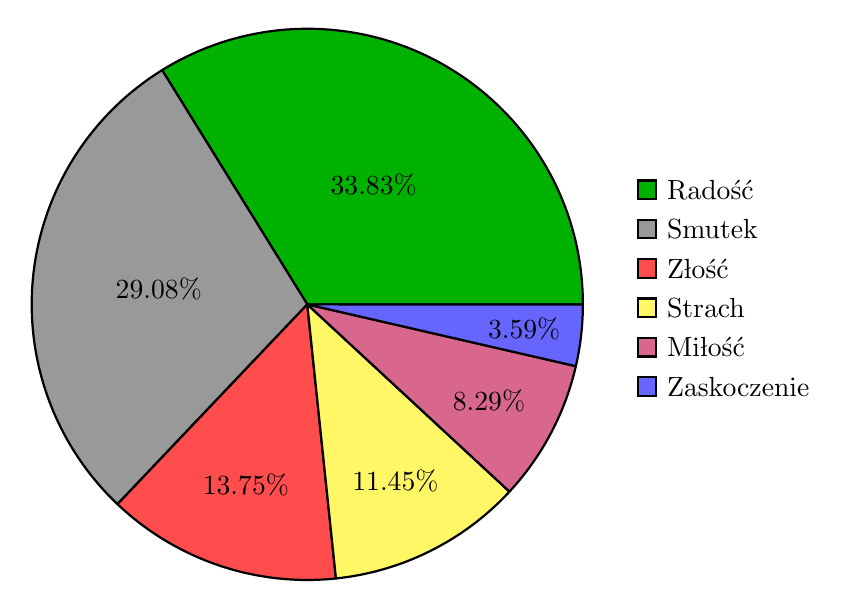
\begin{tikzpicture}
        \pie[text=legend, radius=3.5, color={green!70!black, gray!80, red!70, yellow!60, purple!60, blue!60}]
        {
            33.83/Radość,
            29.08/Smutek,
            13.75/Złość,
            11.45/Strach,
             8.29/Miłość,
             3.59/Zaskoczenie
        }
    \end{tikzpicture}
    \caption{Rozkład procentowy klas w zbiorze do klasyfikacji emocji. Dane własne.}
    \label{fig:emotion-distribution}
\end{figure}

Zbiór danych przeznaczony do klasyfikacji emocji zawierał końcowo 416\,120 wpisów, nie~zawierając przy tym duplikatów czy wartości pustych.

\begin{figure}[H]
    \centering
    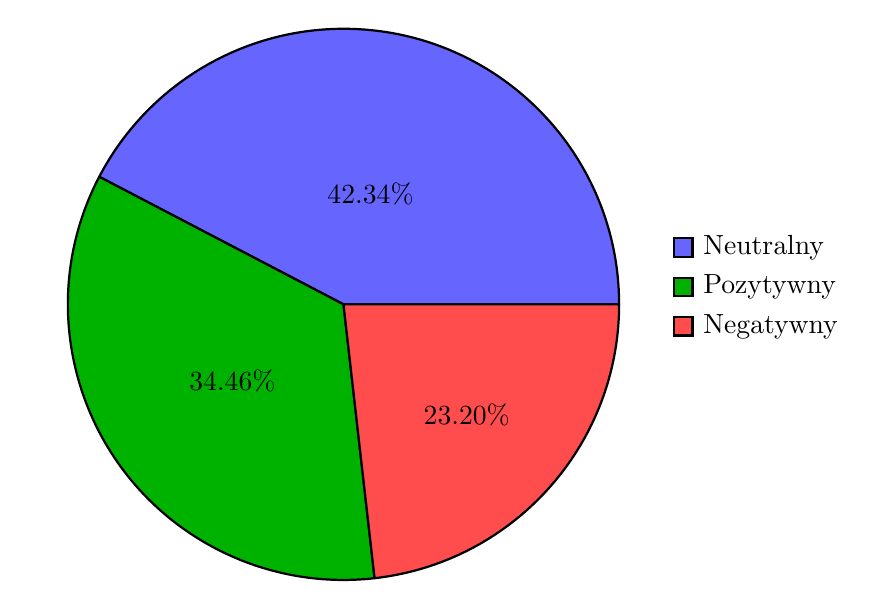
\begin{tikzpicture}
        \pie[text=legend, radius=3.5, color={blue!60, green!70!black, red!70}]
        {
            42.34/Neutralny,
            34.46/Pozytywny,
            23.20/Negatywny
        }
    \end{tikzpicture}
    \caption{Rozkład procentowy klas w zbiorze do klasyfikacji sentymentu. Dane własne.}
    \label{fig:sentiment-distribution}
\end{figure}

Zbiór danych przeznaczony do klasyfikacji sentymentu zawierał 101\,419 wpisów. Po czyszczeniu zaistniała potrzeba usunięcia 150 zduplikowanych rekordów. Finalnie pozostało 101\,269 unikalnych przykładów.

Na tym etapie przetwarzanie danych zostało zakończone, a wszelkie dalsze operacje, takie jak~tokenizacja czy dodanie specjalnych tokenów (np. \textit{[CLS]}, \textit{[SEP]}) wymaganych przez konkretne modele, zostaną przeprowadzone już podczas etapu treningu.

\section{Statystyczna charakterystyka danych po czyszczeniu}

W celu dokładniejszej charakterystyki danych użytych do trenowania modeli przeprowadzono dalszą analizę statystyczną. Analiza skupiła się na rozkładzie klas (w celu oceny nierówności rozkładu w zbiorze i podjęcia działań wyrównujących), długości tekstów oraz częstości występowania słów. Pozwoliło to na identyfikację  ekstremalnych wartości, które mogłyby zaburzyć proces uczenia modeli. Jak piszą autorzy pracy~\cite{ClassImbalance}, niezrównoważone zbiory mogą prowadzić do przetrenowania modeli względem klas dominujących. W takich przypadkach zaleca się zastosowanie technik przeciwdziałających temu zjawisku, takich jak ważenie klas (ang. \textit{class weighting}), nadpróbkowanie lub podpróbkowanie. 

W niniejszej pracy zdecydowano się na zastosowanie mechanizmu ważenia klas, co umożliwia algorytmom lepsze dopasowanie się do mniej licznych klas. Dodatkowo ustalono maksymalną długość tekstu na poziomie 256 znaków, co wynikało z ograniczeń w zasobach obliczeniowych.


\subsection{Zbiór do analizy emocji}
\subsubsection{Rozkład klas}
\begin{figure}[H]
    \centering
    \includegraphics[width=0.7\textwidth]{obrazy/emotion_plot.png}
    \caption{Rozkład liczebności poszczególnych klas w zbiorze danych do analizy emocji. Dane własne.}
    \label{fig:emotion-class-png}
\end{figure}

Na podstawie analizy rozkładu klas (Rysunek \ref{fig:emotion-class-png}) widać wyraźnie, jak nierównomiernie rozkładają się przykłady przypisane do poszczególnych emocji. W celu uzyskania zbioru równomiernego pod względem klas i zgodnego z założoną, dla obu zbiorów, liczbą 100 tysięcy przykładów, z każdej klasy wylosowano maksymalnie 16\,667 przykładów. Jedynym odstępstwem od tej zasady była klasa \textit{„Zaskoczenie”}, której rozmiar nie pozwalał na osiągnięcie docelowej liczby próbek. W związku z tym zdecydowano się również na zastosowanie ważenia klas podczas trenowania modeli.

\subsubsection{Analiza długości tekstów}
\begin{figure}[H]
    \centering
    \includegraphics[width=0.7\textwidth]{obrazy/hist_emotion_1.png}
    \caption{Rozkład długości tekstów w zbiorze danych do analizy emocji. Dane własne.}
    \label{fig:hist-emotion-1-png}
\end{figure}
Powyższy histogram (Rysunek \ref{fig:hist-emotion-1-png}) ukazuje, że znaczna część danych koncentruje się~w~przedziale 50--150 znaków, natomiast najdłuższe wpisy przekraczały 800 znaków. Takie dane odstające mogłyby negatywnie wpłynąć na stabilność trenowania modeli.

\begin{figure}[H]
    \centering
    \includegraphics[width=0.7\textwidth]{obrazy/hist_emotion_2.png}
    \caption{Rozkład długości tekstów w zbiorze danych do analizy emocji o długości poniżej 400 znaków. Dane własne.}
    \label{fig:hist-emotion-2-png}
\end{figure}
Drugi histogram, odfiltrowujący dane o długości równej bądź większej niż 400 znaków (Rysunek \ref{fig:hist-emotion-2-png}), pozwolił na dokładniejsze uwidocznienie struktury rozkładu. Większość wartości mieści się w przedziale od 30 do 120 znaków, jednak pewna część danych rozkłada się również w zakresie od 250 do około 310 znaków.

\begin{figure}[H]
    \centering
    \includegraphics[width=0.7\textwidth]{obrazy/box_emotion_1.png}
    \caption{Rozkład liczby znaków w próbkach w zbiorze do analizy emocji. Dane własne.}
    \label{fig:box-emotion-1-png}
\end{figure}
Na wykresie pudełkowym (Rysunek \ref{fig:box-emotion-1-png}) widać, że wszystkie wartości powyżej 239 znaków można uznać za wartości odstające (outliers). Gdyby wszystkie te próbki były potraktowane jako outliers, ich liczba wynosiłaby 9\,951. Zdecydowano się jednak odciąć jedynie próbki, których długość jest większa niż 256.

\begin{figure}[H]
    \centering
    \includegraphics[width=0.7\textwidth]{obrazy/hist_emotion_3.png}
    \caption{Rozkład długości tekstów w zbiorze danych do analizy emocji po usunięciu wartości odstających. Dane własne.}
    \label{fig:hist-emotion-3-png}
\end{figure}
Po odcięciu 4\,922 rekordów, pozostało 411\,198 próbek. Jak wspomniano wcześniej, największe zagęszczenie danych jest wyraźnie widoczne w przedziale od około 30 do 120 znaków.


\subsubsection{Analiza częstości występowania słów}
Przeprowadzono również analizę najczęściej występujących słów w korpusie, której wyniki zostały zwizualizowane za pomocą chmury słów (ang. \textit{WordCloud}). W pierwszym etapie obliczono najczęściej pojawiające się słowa w całym zbiorze danych. Wśród nich znalazły się kolejno takie wyrazy jak: \textit{„i”, „feel”, „and”, „to”, „the”, „a”, „feeling”, „that”, „of”} oraz \textit{„my”}. Dominacja słów takich jak \textit{„i”} (ja) oraz \textit{„feel”} (czuje) sugeruje, że zbiór danych koncentruje się~na~odczuciach, co może wpłynąć na wyraźne rozróżnienie emocji przez modele klasyfikacyjne.

\begin{figure}[H]
    \centering
    \includegraphics[width=0.9\textwidth]{obrazy/cloud_emotion_1.png}
    \caption{Chmura słow dla zbioru do analizy emocji. Dane własne.}
    \label{fig:cloud-emotion-1-png}
\end{figure}
Na chmurze słów dominują wyrazy związane z emocjami, takie jak \textit{„feel”, „feeling”, „love”, „life”, „happy”}, co również potwierdza sugestję, że~dane koncentrują się~na~odczuciach i~emocjonach.

\newpage
W kolejnym kroku analizy z danych usunięto słowa funkcjonalne (ang. \textit{stop words}). Po~tym zabiegu, najczęściej występującymi słowami były kolejno: \textit{„feel”, „feeling”, „like”, „im”, „really”, „know”, „time”, „get”, „little”} oraz \textit{„people”}. Na pierwszy plan wysunęły się słowa takie jak, \textit{„feeling”, „like”, "little"} czy \textit{"really"}. \textit{„Feeling”} występuje bezpośrednio po \textit{„feel”}, a \textit{„like”} oraz wzmacniające przekaz \textit{„really”} i \textit{„little”} także odgrywają istotną rolę, co znów sugeruje, że dane mogą koncentrować się na konkretnych emocjach.

\begin{figure}[H]
    \centering
    \includegraphics[width=0.9\textwidth]{obrazy/cloud_emotion_2.png}
    \caption{Chmura słow dla zbioru do analizy emocji po usunięciu słów funkcjonalnych. Dane własne.}
    \label{fig:cloud-emotion-2-png}
\end{figure}
Mimo, że po usunięciu \textit{stop words} na wizualizacji pozostały słowa związane z emocjami, takie jak  \textit{„love”}, ogólny obraz sugeruje, że zbiór może obejmować szeroką gamę słów związanych z emocjami, a nie koncentrować się na jednym dominującym zwrocie.

Pomimo przeprowadzonego czyszczenia, w dalszej analizie zachowano  \textit{stop words} w danych wykorzystywanych do treningu modeli. Jak wspomnianio wcześniej, modele NLP, takie jak BERT czy LSTM, skutecznie wykorzystują kontekst zawarty w pisowni oraz elementach gramatycznych, dlatego nadmierne filtrowanie danych tekstowych nie jest konieczne.

\subsection{Zbiór do analizy sentymentu}
\subsubsection{Rozkład klas}
\begin{figure}[H]
    \centering
    \includegraphics[width=0.7\textwidth]{obrazy/sentiment_plot.png}
    \caption{Rozkład liczebności poszczególnych klas w zbiorze danych do analizy sentymentu. Dane własne.}
    \label{fig:sentiment-class-png}
\end{figure}

W zbiorze do analizy sentymentu również występuje znacząca dysproporcja klas, dlatego też~analogicznie do~zbioru związanego z emocjami, w celu zminimalizowania ryzyka przetrenowania względem klas dominujących, zastosowano ważenie klas dla modeli BERT, GRU, LSTM i SVM.

\subsubsection{Analiza długości tekstów}
\begin{figure}[H]
    \centering
    \includegraphics[width=0.7\textwidth]{obrazy/hist_sentiment_1.png}
    \caption{Rozkład długości tekstów w zbiorze danych do analizy sentymentu.\\Dane własne.}
    \label{fig:hist-sentiment-1-png}
\end{figure}

Histogram długości tekstów (Rysunek \ref{fig:hist-sentiment-1-png}) pokazał znaczną rozpiętość -- większość przykładów zawiera od 100 do 200 znaków, jednak najdłuższe wpisy przekraczały 2\,000 znaków. 

\begin{figure}[H]
    \centering
    \includegraphics[width=0.7\textwidth]{obrazy/hist_sentiment_2.png}
    \caption{Rozkład długości tekstów w zbiorze danych do analizy sentymentu o długości poniżej 700 znaków. Dane własne.}
    \label{fig:hist-sentiment-2-png}
\end{figure}

Histogram ukazujący dane zawierające mniej niż 700 znaków (Rysunek \ref{fig:hist-sentiment-2-png}) pozwolił na~dokładniejsze przedstawienie gęstości rozkładu. Większość wartości znajduje się w okolicach 50–130 znaków, podczas gdy zauważalna część danych rozkłada się również w zakresie od~200~do~500~znaków.

\begin{figure}[H]
    \centering
    \includegraphics[width=0.7\textwidth]{obrazy/box_sentiment_1.png}
    \caption{Rozkład liczby znaków w próbkach w zbiorze do analizy sentymentu.\\Dane własne.}
    \label{fig:box-sentiment-1-png}
\end{figure}

Na wykresie pudełkowym (Rysunek \ref{fig:box-sentiment-1-png}) widać, że próbki o długości powyżej 199 znaków można uznać za wartości odstające. Ich liczba wynosi 3\,596. Jak wspomniano wcześniej, zdecydowano się odciąć jedynie dane o długości większej niż 256 znaków.

\begin{figure}[H]
    \centering
    \includegraphics[width=0.7\textwidth]{obrazy/hist_sentiment_3.png}
    \caption{Rozkład długości tekstów w zbiorze danych do analizy sentymentu\\po usunięciu wartości odstających. Dane własne.}
    \label{fig:hist-sentiment-3-png}
\end{figure}

Po tym zabiegu rozkład długości tekstów na histogramie (Rysunek \ref{fig:hist-sentiment-3-png}) ujawnia wyraźne zagęszczenie w przedziale 50--140 znaków, co jest typowe dla komentarzy internetowych. W wyniku przetwarzania usunięto 2\,590 rekordów, pozostawiając 98\,679 przykładów, co jest zbliżone do planowanej liczby stu tysięcy.

\subsubsection{Analiza częstości występowania słów}
Najczęściej pojawiające się słowa w zbiorze dla sentymentu to kolejno: \textit{„the”, „to”, „I”, „a”, „and”, „in”, „of”, „on”, „is”} oraz \textit{„for”}. Dominują tu słowa funkcjonalne.

\begin{figure}[H]
    \centering
    \includegraphics[width=0.9\textwidth]{obrazy/cloud_sentiment_1.png}
    \caption{Chmura słow dla zbioru do analizy sentymentu. Dane własne.}
    \label{fig:cloud-sentiment-1-png}
\end{figure}
Na chmurze słów dominują wyrazy takie jak \textit{„tomorrow”, „day”, „may”, „will”} i \textit{„now”}, ale~pojawiły się także słowa, które niosą pewną wartość wiązaną z sentymentem, takie~jak~\textit{„best”, „good”, „awesome”} czy \textit{„love”}. Choć bez kontekstu trudno jednoznacznie określić, jak~są~nacechowane wypowiedzi zawierające te słowa, to jednak ich obecność wskazuje na możliwą emocjonalną treść.

Po usunięciu \textit{stop words} najczęściej występującymi słowami były kolejno: \textit{„may”, „Im”, „like”, „tomorrow”, „get”, „going”, „see”, „day”, „time” oraz „go”}.

\begin{figure}[H]
    \centering
    \includegraphics[width=0.9\textwidth]{obrazy/cloud_sentiment_2.png}
    \caption{Chmura słow dla zbioru do analizy sentymentu po usunięciu słów funkcjonalnych. Dane własne.}
    \label{fig:cloud-sentiment-2-png}
\end{figure}

Wyniki pozostały zbliżone do poprzednich. Podobnie jak w przypadku zbioru do analizy emocji, w zbiorze do analizy sentymentu zdecydowano się również na zachowanie \textit{stop words} w~danych wykorzystywanych do treningu.

\section{Podział danych na zestawy treningowe, walidacyjne i testowe}

W celu zapewnienia rzetelnej oceny skuteczności zastosowanych modeli klasyfikacyjnych, a także monitorowania ich procesu uczenia, oba zbiory danych zostały podzielone na trzy niezależne zestawy: treningowy, walidacyjny oraz testowy. 

Zbiór danych do analizy sentymentu został podzielony w proporcji 70\% / 15\% / 15\%, odpowiednio dla zestawu treningowego, walidacyjnego i testowego. Podział został wykonany w~sposób losowy, przy zastosowaniu ustalonego ziarna losowości. Aby zagwarantować reprezentatywność każdego z podzbiorów, zastosowano stratyfikację względem etykiet klas -- oznacza to, że proporcje klas (negatywna, neutralna, pozytywna) w każdym z podzbiorów odpowiadają proporcjom występującym w całym zbiorze. Wszystkie uzyskane podzbiory zostały zapisane i~w~dalszych etapach eksperymentów wykorzystano je niezmiennie dla każdego z modeli klasyfikacyjnych analizujących sentyment.

Analogiczne podejście zastosowano przy przygotowywaniu danych dla zadania klasyfikacji emocji, przy czym dodatkowo, przed dokonaniem podziału, zbiór został zrównoważony pod~względem liczebności klas. Zastosowano próbkowanie z zachowaniem równych udziałów, tzn.~dla~każdej z~klas (z wyjątkiem najmniej licznej -- „zaskoczenie”) losowo wybrano po 16\,667 przykładów ($16\,667 \times 6 \approx 100\,000$). 

W niniejszej pracy nie zastosowano walidacji krzyżowej, co było celowym wyborem metodologicznym wynikającym z potrzeby zapewnienia spójności porównania pomiędzy różnymi modelami, które znacząco różnią się pod względem złożoności oraz czasu trenowania, zwłaszcza w przypadku modeli transformatorowych, takich jak BERT, dla których proces treningu jest czasochłonny. Wykorzystany stały, stratyfikowany podział na zbiory treningowy, walidacyjny i~testowy umożliwił jednoznaczną i powtarzalną ocenę skuteczności modeli. Pozwoliło to na porównanie modeli w ich podstawowej konfiguracji, bez wprowadzania dodatkowej optymalizacji hiperparametrów, ponieważ celem badania nie było maksymalne dostosowanie każdego modelu indywidualnie.

\endinput
\chapter{Modele i metody treningu}
W tym rozdziale przedstawione zostaną opisy modeli wykorzystanych w pracy, uwzględniając ich architekturę, cechy charakterystyczne oraz sposób treningu. Celem jest omówienie procesu uczenia tych modeli, a także przedstawienie parametrów, które zostały użyte podczas trenowania. W tym przypadku starano się zachować jak najmniejszą ingerencję w ustawienia modeli, by przeprowadzić porównanie samych algorytmów, a nie ich dostosowanych wersji, które mogłyby wymagać indywidualnego dostrajania hiperparametrów dla każdego modelu. Modele były trenowane w ten sam sposób zarówno dla klasyfikacji sentymentu, jak i emocji, dlatego opisy dotyczące procesów treningu nie będą powtarzane dla każdej z tych kategorii osobno.

\section{Model SVM}
Głównym celem maszyny wektorów nośnych jest znalezienie hiperpowierzchni (w przestrzeni cech), która maksymalizuje margines pomiędzy różnymi klasami. W klasyfikacji binarnej SVM stara się znaleźć prostą, która najlepiej separuje dwie klasy, zachowując jak największy odstęp (margines) od punktów należących do tych klas~\cite{UczMasz}.

W klasyfikacji wieloklasowej, jak ma to miejsce w analizie sentymentu i emocji, gdzie w tym przypadku najmniejsza liczba klas wynosi trzy, algorytm SVM stosuje podejście rozszerzające model do obsługi większej liczby etykiet. Zamiast klasycznego podejścia binarnego, wykorzystuje się różne strategie. W pracy tej zastosowano metodę \textit{„jeden kontra jeden”} (ang. \textit{One-vs-One}, OvO). W tej metodzie dla każdej pary klas tworzony jest osobny klasyfikator, a każdy z tych klasyfikatorów wyznacza hiperpłaszczyznę, która oddziela te dwie klasy.

Klasyfikując sentyment, szczególnie ważnym elementem jest przekształcenie danych tekstowych do postaci, którą model może analizować w przestrzeni cech. Tekst, który jest z natury sekwencyjny i nieliczbowy, musi zostać odpowiednio przetworzony, aby mógł być użyty w algorytmie. W tym celu stosuje się odpowiednie techniki reprezentacji tekstu, jak chociażby TF-IDF, o którym mowa poniżej.

\subsection{Zastosowana implementacja i parametry}
W pracy wykorzystano implementację modelu SVM z biblioteki scikit-learn~\cite{SKLearnSVM}. Implementacja ta została użyta z domyślnymi parametrami, z wyjątkiem kilku zmian, które zostały opisane poniżej.

Do reprezentacji tekstu w przestrzeni cech zastosowano TF-IDF (\textit{Term Frequency-Inverse Document Frequency}), który przekształca słowa w wektory, uwzględniając częstotliwość występowania słów w danej próbce oraz ich istotność w kontekście całego zbioru danych. W procesie tokenizacji wybrano 20\,000 najczęściej występujących słów w zbiorze, które zostały potraktowane jako cechy wejściowe dla modelu. Dzięki temu słowa w zbiorze tekstów są reprezentowane jako liczby, które model SVM wykorzystuje do klasyfikacji.

Model SVM został użyty z jądrem liniowym. Jest to najprostszy kernel, który jest także wydajny w klasyfikacji tekstu. W badaniu~\cite{KernelComparison} stwierdzono, że jądro liniowe osiąga najwyższą dokładność klasyfikacji w najkrótszym czasie. 

Zastosowano ważenie klas, które miało na celu zrównoważenie nierównomiernego rozkładu danych, omówionego w poprzednim rozdziale. Dzięki temu model miał szansę lepiej poradzić sobie z klasami występującymi rzadziej, minimalizując dominację bardziej reprezentowanych klas w zbiorze treningowym.

Parametr C, ustawiony został na wartość 1.0. Pełni on rolę regularyzacji, balansując pomiędzy dopasowaniem modelu do danych a jego zdolnością do generalizacji. Wyższe wartości C zmniejszają margines błędu, co może prowadzić do przeuczenia, natomiast niższe wartości zwiększają tolerancję na błąd, sprzyjając lepszemu uogólnianiu~\cite{UczMasz}.

\subsection{Proces treningu}
W standardowej implementacji w bibliotece scikit-learn algorytm SVM jest zoptymalizowany do pracy na CPU, dlatego model nie był trenowany na GPU. Czas trenowania wyniósł około 5--7 minut zarówno dla klasyfikacji sentymentu, jak i emocji. Czasy treningu przedstawione w~tej~pracy służą głównie do porównań między modelami, a nie do wyciągania dalszych wniosków.

W analizie sentymentu model osiągnął średnią dokładność 66\% na zbiorze testowym i 65\% na walidacyjnym, co wskazuje na dobre dopasowanie, ponieważ wyniki są porównywalne, sugerując brak przetrenowania i niedotrenowania. Niska dokładność może wynikać z samej natury zadania oraz złożoności tekstów.

W klasyfikacji emocji model uzyskał dokładność 91\% zarówno na zbiorze testowym, jak~i~walidacyjnym, co~świadczy o dobrym dopasowaniu i wysokiej skuteczności, a także sugeruje, że~model dobrze generalizuje lub teksty były wyraźnie zróżnicowane.

\section{Model LSTM}
\textit{Long Short-Term Memory} (LSTM) to rodzaj rekurencyjnej sieci neuronowej (RNN), który został zaprojektowany do rozwiązania problemu zanikania gradientu, występującego w klasycznych RNN podczas trenowania na długich sekwencjach. Dzięki swojej strukturze, LSTM jest~w~stanie przechowywać istotne informacje przez dłuższy czas, co sprawia, że świetnie nadaje się do analizy sekwencji, takich jak teksty. W LSTM wykorzystywane są trzy bramki: wejściowa, zapomnienia oraz wyjściowa, które pozwalają modelowi kontrolować przepływ informacji oraz zapamiętywać lub zapominać ważne lub nieistotne dane w zależności od kontekstu. Dzięki tym mechanizmom LSTM jest w stanie uchwycić długoterminowe zależności w danych, co czyni go~odpowiednim narzędziem w analizie tekstów~\cite{LSTMIntroduction}.

\subsection{Zastosowana implementacja i parametry}
Implementacja modelu LSTM w tej pracy opiera się na bibliotece PyTorch, która oferuje dużą elastyczność w implementacji sieci neuronowych oraz zapewnia dostęp do narzędzi do~ich~treningu i~ewaluacji~\cite{PyTorchDocs}. W tej pracy użyto modelu LSTM z 256 jednostkami w warstwie ukrytej, z dodatkową warstwą osadzającą (ang. \textit{embedding layer}), która przekształca tokeny na~wektory o wymiarze 256.

\newpage
Do tokenizacji tekstów użyto narzędzia z biblioteki Keras~\cite{KerasDocs}. Proces tokenizacji polega na~przekształceniu tekstów w sekwencje liczb (tokeny), które mogą być użyte w modelu. W~przypadku tej implementacji podobnie jak w przypadku modelu SVM również wybierano 20\,000 najczęściej występujących słów w zbiorze danych.

Początkowa implementacja modelu, zarówno dla klasyfikacji emocji, jak i sentymentu, wykazała problem z nadmiernym dopasowaniem do tylko i wyłącznie jednej klasy. Aby poprawić wyniki, zastosowano warstwę dropout o współczynniku 0.5. Dropout jest techniką regularyzacji, która polega na losowym wyłączaniu części neuronów podczas treningu, co pozwala na~zwiększenie ogólnej zdolności modelu do generalizacji na nowych danych. Dodatkowo, w celu poprawy efektywności przetwarzania tekstu, użyto dwukierunkowego LSTM (ang. \textit{bidirectional LSTM}). Implementacja modelu LSTM objęła także wykorzystanie funkcji aktywacji ReLU (ang. \textit{Rectified Linear Unit}) w warstwie wyjściowej. 

Cała sieć została zoptymalizowana przy użyciu algorytmu Adam (ang. \textit{Adaptive Moment Estimation}), który jest jedną z popularniejszych metod optymalizacji w uczeniu głębokich sieci neuronowych. W celu zrównoważenia nierównomiernego rozkładu danych w zbiorze treningowym wprowadzono wagi klasowe.

W przypadku wersji wielozadaniowej model był trenowany równolegle do obu zadań. Dwie oddzielne warstwy wyjściowe zostały użyte do klasyfikacji sentymentu i emocji.

\subsection{Proces treningu}
Model LSTM był trenowany przez dwie epoki, co zostało uznane za standard dla wszystkich modeli po testach na modelu BERT. Taka długość treningu okazała się wystarczająca do uzyskania stabilnych wyników oraz zapobiegła przeuczeniu. Czas treningu wynosił średnio 10 minut dla~wersji jednozadaniowych, a dla wersji multitask około 20 minut. Modele były trenowane na~GPU.

\begin{table}[H]
\centering
\label{tab:lstm_training_process}
\begin{tabular}{|l|c|c|c|c|}
\hline
\textbf{Epoka} & \multicolumn{2}{c|}{\textbf{Sentyment}} & \multicolumn{2}{c|}{\textbf{Emocje}} \\
\cline{2-5}
& \textbf{Dokł. (train)} & \textbf{Dokł (val)} & \textbf{Dokł (train)} & \textbf{Dokł (val)} \\
\hline
1 & 55.27\% & 63.04\% & 67.27\% & 92.06\% \\
2 & 68.24\% & 66.68\% & 93.34\% & 94.76\% \\
\hline
\end{tabular}
\caption{Porównanie dokładności podczas treningu modeli jednozadaniowych LSTM.\\Dane własne.}
\end{table}

W przypadku wersji jednozadaniowej, dla klasyfikacji sentymentu model uzyskał dokładność 67\% na zbiorze testowym, 68\% na zbiorze treningowym oraz 66.7\% na zbiorze walidacyjnym. Z danych przedstawionych w tabeli powyżej widać, że model poprawiał wyniki na zbiorze treningowym i walidacyjnym w procesie uczenia.

W analizie emocji model osiągnął dokładność 96.7\% na zbiorze testowym, 93\% na zbiorze treningowym oraz niemal 95\% na zbiorze walidacyjnym, co sugeruje skuteczną klasyfikację. W~trakcie procesu treningowego również nie zauważono oznak przeuczenia.

\begin{table}[H]
\centering
\label{tab:lstm_multi_training_process}
\begin{tabular}{|l|c|c|c|c|}
\hline
\textbf{Epoka} & \multicolumn{2}{c|}{\textbf{Sentyment}} & \multicolumn{2}{c|}{\textbf{Emocje}} \\
\cline{2-5}
& \textbf{Dokł. (train)} & \textbf{Dokł. (val)} & \textbf{Dokł. (train)} & \textbf{Dokł. (val)} \\
\hline
1 & 54.11\% & 64.53\% & 71.31\% & 93.57\% \\
2 & 66.93\% & 66.13\% & 93.92\% & 94.54\% \\
\hline
\end{tabular}
\caption{Porównanie dokładności podczas treningu modelu wielozadaniowego LSTM.\\Dane własne.}
\end{table}

W przypadku modelu wielozadaniowego proces treningu przebiegał bardzo podobnie, osiągając niemal identyczne wyniki jak modele jednozadaniowe dla obu zadań.

\section{Model GRU}
\textit{Gated Recurrent Units} (GRU) to kolejny typ rekurencyjnej sieci neuronowej, który, podobnie jak LSTM, został zaprojektowany w celu rozwiązania problemu zanikania gradientu. GRU~różni się od LSTM tym, że posiada jedynie dwie bramki: bramkę aktualizacji oraz bramkę zapomnienia. Bramka aktualizacji decyduje, jakie informacje mają zostać zachowane, a bramka zapomnienia określa, które informacje należy zapomnieć. Dzięki tej uproszczonej strukturze, GRU~jest szybsze w trenowaniu i potrzebuje mniej zasobów obliczeniowych, jednocześnie osiągając zbliżoną skuteczność w porównaniu do LSTM w wielu zadaniach, w tym w analizie tekstu~\cite{GRUvsLSTM}.

\subsection{Zastosowana implementacja i parametry} 
W przypadku GRU implementacja również opiera się o bibliotekę PyTorch~\cite{PyTorchDocs}. Implementacja jest bliźniaczo podobna: model wykorzystuje warstwę osadzającą, która przekształca tokeny na wektory o wymiarze 256, a następnie przechodzi przez warstwę GRU z 256 jednostkami ukrytymi. Proces tokenizacji przebiegł dokładnie tak samo jak w przypadku modelu LSTM. Użyto tokenizera z biblioteki Keras~\cite{KerasDocs} i wybrano 20\,000 najczęściej występujących słów w~zbiorze.

Różnice między modelami LSTM i GRU pojawiają się w tym miejscu. Dla standardowych, powyższych ustawień model GRU osiągnął wyniki porównywalne do tych, które uzyskano po~wprowadzeniu dodatkowych parametrów. Dodatkowe parametry zostały wprowadzone w celu zapewnienia sprawiedliwego porównania między modelami. Zastosowano więc również warstwę dropout o współczynniku 0.5. Użyto również dwukierunkowego GRU (ang. \textit{bidirectional GRU}), który tak jak dla modelu LSTM umożliwia modelowi analizowanie tekstu zarówno od~lewej do~prawej, jak i~od~prawej do~lewej. W warstwie wyjściowej zastosowano funkcję aktywacji ReLU, a optymalizacja modelu przebiegała z wykorzystaniem algorytmu Adam. Tak~jak~w~przypadku LSTM, również w tym modelu użyto wag klasowych.

Wersja wielozadaniowa modelu GRU była trenowana paralelnie do obu zadań -- klasyfikacji sentymentu oraz emocji. Do każdego z tych zadań przypisano oddzielną warstwę wyjściową.

\newpage
\subsection{Proces treningu} 
Trening modelu GRU obejmował dwie epoki, a czas treningu był bardzo zbliżony do modelu LSTM i również wynosił około 10 minut dla wersji jednozadaniowych oraz około 20 minut dla~modelu wielozadaniowego. Trening odbywał się na procesorze graficznym.

\begin{table}[H]
\centering
\label{tab:gru_training_process}
\begin{tabular}{|l|c|c|c|c|}
\hline
\textbf{Epoka} & \multicolumn{2}{c|}{\textbf{Sentyment}} & \multicolumn{2}{c|}{\textbf{Emocje}} \\
\cline{2-5}
& \textbf{Dokł. (train)} & \textbf{Dokł. (val)} & \textbf{Dokł. (train)} & \textbf{Dokł. (val)} \\
\hline
1 & 55.20\% & 64.28\% & 76.35\% & 94.22\% \\
2 & 67.95\% & 64.38\% & 93.87\% & 94.33\% \\
\hline
\end{tabular}
\caption{Porównanie dokładności podczas treningu modeli jednozadaniowych GRU.\\Dane własne.}
\end{table}

Klasyfikując sentyment model uzyskał dokładność na poziomie 64\% na zbiorze testowym, 68\% na zbiorze treningowym oraz 64\% na zbiorze walidacyjnym. Analizując wyniki na zbiorze walidacyjnym w trakcie procesu uczenia, można zauważyć, że dokładność stabilizuje się, co~wskazuje na pewną stagnację w dalszym uczeniu modelu. Niemniej jednak, model nie wykazuje oznak przeuczenia, ponieważ dokładność na zbiorze walidacyjnym nie spadła, mimo wzrostu wydajności na zbiorze treningowym.

W analizie emocji, model osiągnął dokładność na poziomie 94\% na zbiorze testowym, niemal 94\% na zbiorze treningowym oraz 94\% na zbiorze walidacyjnym. Również w tym przypadku wyniki są stabilne, ale model nie wykazuje oznak przeuczenia.

\begin{table}[H]
\centering
\label{tab:gru_multi_training_process}
\begin{tabular}{|l|c|c|c|c|}
\hline
\textbf{Epoka} & \multicolumn{2}{c|}{\textbf{Sentyment}} & \multicolumn{2}{c|}{\textbf{Emocje}} \\
\cline{2-5}
& \textbf{Dokł. (train)} & \textbf{Dokł. (val)} & \textbf{Dokł. (train)} & \textbf{Dokł. (val)} \\
\hline
1 & 54.38\% & 63.41\% & 77.53\% & 94.12\% \\
2 & 66.92\% & 64.98\% & 93.77\% & 94.36\% \\
\hline
\end{tabular}
\caption{Porównanie dokładności podczas treningu modelu wielozadaniowego GRU.\\Dane własne.}
\end{table}

Proces treningu modelu wielozadaniowego przebiegał w sposób zbliżony do modeli jednozadaniowych, osiągając prawie takie same wyniki dla obu zadań.

\section{Model BERT}
\textit{Bidirectional Encoder Representations from Transformers} (BERT) to najbardziej zaawansowany model użyty w tej pracy, a także jeden z najbardziej zaawansowanych modeli w dziedzinie przetwarzania języka naturalnego. Model ten bazuje na architekturze Transformer, która wykorzystuje mechanizm \textit{self-attention} do przetwarzania sekwencji. Główna innowacja BERT-a polega na jego dwukierunkowym podejściu do analizy tekstu, co oznacza, że~model uwzględnia kontekst zarówno poprzedzających, jak i następujących słów w~danym zdaniu. Jednak w~przeciwieństwie do LSTM czy GRU, które realizują dwukierunkowość poprzez analizowanie tekstu sekwencyjnie, BERT wykorzystuje wspomniany wcześniej mechanizm samouwagi, który pozwala mu jednocześnie analizować całą sekwencję, uwzględniając kontekst wszystkich słów w~zdaniu. To umożliwia modelowi lepsze uchwycenie semantycznych relacji między słowami~\cite{BERT}.

BERT jest wstępnie przetrenowany na ogromnych zbiorach danych, co pozwala na uzyskanie uniwersalnych reprezentacji słów, które mogą być później dostosowane do różnych zadań za~pomocą dodatkowego etapu \textit{fine-tuningu}. W praktyce oznacza to, że model BERT może być łatwo zaadoptowany do szerokiego zakresu zadań NLP, w tym właśnie analizy sentymentu czy rozpoznawania emocji.

\subsection{Zastosowana implementacja i parametry}

W tej pracy użyto implementacji modelu BERT dostępnej w bibliotece Hugging Face transformers~\cite{HuggingFaceDocs}. Model oparty jest na wersji \textit{bert-base-uncased}, która została wstępnie przetrenowana na dużych zbiorach danych i dostosowana do klasyfikacji tekstów. Użyto tokenizera BERT z~tej~samej biblioteki, a w procesie tokenizacji wszystkie słowa zostały przekształcone na tokeny, a teksty zostały przycięte lub uzupełnione do maksymalnej długości 256 tokenów.

Wszystkie modele, zarówno jednozadaniowe, jak i wielozadaniowe, używały tych samych parametrów, aby zapewnić sprawiedliwe porównanie. Model BERT w użytej wersji implementacji oparty jest na 12 ukrytych warstwach transformera. Długość sekwencji wejściowej została ustalona na 256 tokenów. Liczba epok wynosiła początkowo pięć, jednak po analizie wyników stwierdzono, że model zaczyna się przetrenowywać po drugiej epoce, dlatego ostatecznie zdecydowano się na dwie epoki. Optymalizacja modelu odbywała się za pomocą algorytmu AdamW, który jest dostosowaną wersją algorytmu Adam, przystosowaną do pracy z parametrami BERT-a. Funkcja strat to \textit{Cross-Entropy Loss}, z wagami klasowymi, które zostały obliczone na podstawie nierównomiernego rozkładu klas w zbiorze treningowym.

Wersja wielozadaniowa modelu BERT wykorzystywała dwie oddzielne warstwy wyjściowe: jedną do klasyfikacji sentymentu i drugą do klasyfikacji emocji. 

\subsection{Proces treningu}
\raggedbottom
\vspace{20pt}
\begin{table}[H]
\centering
\label{tab:bert_5_training_process}
\begin{tabular}{|l|c|c|c|c|}
\hline
\textbf{Epoka} & \multicolumn{2}{c|}{\textbf{Sentyment}} & \multicolumn{2}{c|}{\textbf{Emocje}} \\
\cline{2-5}
& \textbf{Dokł. (train)} & \textbf{Dokł. (val)} & \textbf{Dokł. (train)} & \textbf{Dokł. (val)} \\
\hline
1 & 70.77\% & 72.92\% & 91.48\% & 95.18\% \\
2 & 79.13\% & 73.41\% & 94.94\% & 95.24\% \\
3 & 87.32\% & 72.93\% & 95.10\% & 95.10\% \\
4 & 92.89\% & 72.07\% & 95.32\% & 95.24\% \\
5 & 95.35\% & 72.61\% & 95.43\% & 95.04\% \\
\hline
\end{tabular}
\caption{Porównanie dokładności podczas treningu na pięciu epokach modeli jednozadaniowych BERT. Dane własne.}
\end{table}

\begin{table}[H]
\centering
\label{tab:bert_multi_5_training_process}
\begin{tabular}{|l|c|c|c|c|}
\hline
\textbf{Epoka} & \multicolumn{2}{c|}{\textbf{Sentyment}} & \multicolumn{2}{c|}{\textbf{Emocje}} \\
\cline{2-5}
& \textbf{Dokł. (train)} & \textbf{Dokł. (val)} & \textbf{Dokł. (train)} & \textbf{Dokł. (val)} \\
\hline
1 & 69.85\% & 72.86\% & 91.19\% & 94.99\% \\
2 & 77.60\% & 72.24\% & 94.85\% & 94.89\% \\
3 & 85.17\% & 72.13\% & 95.17\% & 95.11\% \\
4 & 90.85\% & 71.64\% & 95.24\% & 95.05\% \\
5 & 93.71\% & 71.26\% & 95.36\% & 95.23\% \\
\hline
\end{tabular}
\caption{Porównanie dokładności podczas treningu na pięciu epokach modelu wielozadaniowego BERT. Dane własne.}
\end{table}

W pierwszym podejściu model BERT był trenowany przez pięć epok, zarówno dla wersji jednozadaniowych, jak i wielozadaniowych. Po przeanalizowaniu wyników na zbiorze walidacyjnym zauważono, że po pewnym czasie dokładność modelu na zbiorze walidacyjnym zaczynała się stabilizować lub wręcz maleć. Takie zachowanie wskazywało na problem z przeuczeniem, szczególnie w przypadku wersji jednozadaniowej dla klasyfikacji sentymentu. Podobny trend~zauważono w wersji wielozadaniowej, gdzie dokładność na zbiorze walidacyjnym również malała.

W związku z tym, zdecydowano, że liczba epok będzie ograniczona do dwóch. Takie podejście miało na celu uniknięcie przeuczenia. Zmniejszenie liczby epok okazało się skuteczne, a~czas treningu został skrócony. Trening modelu BERT na pięciu epokach trwał średnio dwie godziny dla wersji jednozadaniowej i około pięć godzin dla wersji wielozadaniowej. Wszystkie modele były trenowane na GPU.

\begin{table}[H]
\centering
\label{tab:bert_2_training_process}
\begin{tabular}{|l|c|c|c|c|}
\hline
\textbf{Epoka} & \multicolumn{2}{c|}{\textbf{Sentyment}} & \multicolumn{2}{c|}{\textbf{Emocje}} \\
\cline{2-5}
& \textbf{Dokł. (train)} & \textbf{Dokł. (val)} & \textbf{Dokł. (train)} & \textbf{Dokł. (val)} \\
\hline
1 & 70.64\% & 73.61\% & 91.25\% & 95.10\% \\
2 & 78.91\% & 73.69\% & 94.92\% & 95.14\% \\
\hline
\end{tabular}
\caption{Porównanie dokładności podczas treningu modeli jednozadaniowych BERT.\\Dane własne.}
\end{table}

\begin{table}[H]
\centering
\label{tab:bert_multi_2_training_process}
\begin{tabular}{|l|c|c|c|c|}
\hline
\textbf{Epoka} & \multicolumn{2}{c|}{\textbf{Sentyment}} & \multicolumn{2}{c|}{\textbf{Emocje}} \\
\cline{2-5}
& \textbf{Dokł. (train)} & \textbf{Dokł. (val)} & \textbf{Dokł. (train)} & \textbf{Dokł. (val)} \\
\hline
1 & 69.58\% & 72.96\% & 91.06\% & 94.79\% \\
2 & 77.71\% & 72.47\% & 94.82\% & 94.97\% \\
\hline
\end{tabular}
\caption{Porównanie dokładności podczas treningu modelu wielozadaniowego BERT.\\Dane własne.}
\end{table}

W drugim podejściu, czas treningu modelu BERT na wersji jednozadaniowej wynosił średnio jedną godzinę, podczas gdy dla wersji wielozadaniowej trwał około dwóch godzin. W przypadku klasyfikacji sentymentu, model uzyskał dokładność 74\% na zbiorze testowym, 72\% na zbiorze walidacyjnym oraz 78\% na zbiorze treningowym. Wyniki te wskazują, że model jest właściwie dopasowany, choć na zbiorze walidacyjnym i testowym wystąpił pewien spadek dokładności w~porównaniu do zbioru treningowego, co może sugerować lekkie przeuczenie. Natomiast w~analizie emocji model osiągnął bardzo wysoką dokładność 95\% zarówno na zbiorze walidacyjnym, jak i testowym, a na zbiorze treningowym wynik ten był niemal identyczny, co sugeruje, że~model dobrze radzi sobie z klasyfikacją emocji i nie jest przetrenowany.

W przypadku wersji wielozadaniowej, wyniki były porównywalne.

\section{Reprodukcja wyników}
Kod źródłowy wykorzystany do przeprowadzenia eksperymentów oraz treningu wszystkich modeli jest dostępny pod adresem: \url{https://github.com/Primuu/MastersThesis}. Repozytorium zawiera dane, skrypty do przygotowania danych, implementacje modeli, procesy treningowe oraz skrypty do ewaluacji i wizualizacji wyników.

Wszystkie eksperymenty były realizowane z użyciem bibliotek:
\begin{itemize}
    \item \texttt{pandas} -- wersja 2.2.3,
    \item \texttt{scikit-learn} -- wersja 1.5.2,
    \item \texttt{PyTorch} -- wersja 2.4,
    \item \texttt{transformers} -- wersja 4.46.2,
    \item \texttt{tensorflow} -- wersja 2.10,
    \item \texttt{matplotlib} -- wersja 3.9.2,
    \item \texttt{seaborn} -- wersja 0.13.
\end{itemize}

\section{Miary skuteczności}
Wszystkie modele zostały ocenione przy użyciu czterech miar: \textit{accuracy}, \textit{precision}, \textit{recall} oraz \textit{F1-score}. 
\begin{itemize}
    \item \textit{Accuracy} (dokładność) oblicza się jako stosunek liczby poprawnych klasyfikacji do całkowitej liczby próbek. W przypadku niezrównoważonych klas może nie oddać pełnej skuteczności modelu.
    \item \textit{Precision} (precyzja) mierzy, ile z przewidywanych pozytywnych przypadków jest faktycznie pozytywnych. Wysoka precyzja oznacza, że model rzadko popełnia błędy.
    \item \textit{Recall} (czułość) mierzy, ile z rzeczywistych pozytywnych przypadków zostało poprawnie zidentyfikowanych przez model.
    \item \textit{F1-score} to średnia harmoniczna między precyzją a czułością, która pozwala na uzyskanie zrównoważonego wyniku. F1-score jest szczególnie użyteczne w przypadkach, gdy klasy są~niezrównoważone, ponieważ traktuje precyzję i czułość w równym stopniu.
\end{itemize}

\endinput
\chapter{Eksperymenty i wyniki}

Celem tego rozdziału jest zaprezentowanie wyników uzyskanych w trakcie przeprowadzonych eksperymentów. Jak zostało wpsomniane, analizowane były trzy zadania: klasyfikacja sentymentu, klasyfikacja emocji oraz jednoczesna klasyfikacja sentymentu i emocji. W pierwszej kolejności omówione zostaną wyniki uzyskane przez modele jednozadaniowe, a następnie zestawione zostaną ich osiągi z modelami wielozadaniowymi.

\section{Modele jednozadaniowe dla analizy sentymentu}
W zadaniu klasyfikacji sentymentu przetestowano cztery różne architektury: BERT, LSTM, GRU oraz klasyfikator SVM.

\begin{table}[H]
\centering
\label{tab:sentiment_models}
\begin{tabular}{|l|c|c|c|c|}
\hline
\textbf{Model} & \textbf{Dokł.} & \textbf{Prec. (makro)} & \textbf{Czuł. (makro)} & \textbf{F1-score (makro)} \\
\hline
BERT & 0.74 & 0.74 & 0.74 & 0.74 \\
LSTM & 0.67 & 0.67 & 0.68 & 0.67 \\
GRU  & 0.64 & 0.64 & 0.67 & 0.64 \\
SVM  & 0.66 & 0.65 & 0.66 & 0.66 \\
\hline
\end{tabular}
\caption{Zestawienie miar skuteczności dla modeli jednozadaniowych w zadaniu klasyfikacji sentymentu. Dane własne.}
\end{table}

Model BERT uzyskał najwyższe wyniki we wszystkich czterech miarach, osiągając 0.74~zarówno w dokładności, jak i w precyzji, czułości oraz \textit{F1-score}. Oznacza to, że model ten najskuteczniej radził sobie z klasyfikacją wszystkich klas sentymentu w sposób zrównoważony.

Model LSTM uplasował się na drugim miejscu, osiągając dokładność 0.67 oraz zbliżone wartości pozostałych miar. Wskazuje to na stabilną, choć niższą niż BERT, skuteczność klasyfikacji.

Model SVM uzyskał dokładność 0.66, a pozostałe miary także utrzymywały się na podobnym poziomie, co świadczy o jego spójności w przewidywaniu klas, mimo że nie wykorzystuje mechanizmów głębokiego uczenia.

Model GRU osiągnął najniższe wartości, co sugeruje, że był najmniej skuteczny w klasyfikacji spośród porównywanych modeli jednozadaniowych.

\newpage
\section{Modele jednozadaniowe dla analizy emocji}

W zadaniu identyfikacji emocji wykorzystano te same architektury, które były użyte przy klasyfikacji sentymentu, czyli: BERT, LSTM, GRU oraz SVM.

\begin{table}[H]
\centering
\label{tab:emotion_models}
\begin{tabular}{|l|c|c|c|c|}
\hline
\textbf{Model} & \textbf{Dokł.} & \textbf{Prec. (makro)} & \textbf{Czuł. (makro)} & \textbf{F1-score (makro)} \\
\hline
BERT & 0.95 & 0.95 & 0.95 & 0.95 \\
LSTM & 0.95 & 0.95 & 0.95 & 0.95 \\
GRU  & 0.94 & 0.94 & 0.94 & 0.94 \\
SVM  & 0.91 & 0.91 & 0.91 & 0.91 \\
\hline
\end{tabular}
\caption{Zestawienie miar skuteczności dla modeli jednozadaniowych w zadaniu klasyfikacji emocji. Dane własne.}
\end{table}

Model BERT osiągnął najwyższe wyniki spośród wszystkich analizowanych modeli, uzyskując wartość 0.95 we wszystkich czterech miarach: dokładności, precyzji, czułości oraz \textit{F1-score}. Choć model LSTM osiągnął identyczne wartości w tej zbiorczej tabeli, to BERT uzyskał wyższe wyniki dla większości poszczególnych klas emocji, co czyni go obiektywnie lepszym modelem w tym zadaniu. Różnice te zostaną przedstawione w sekcji niżej, poświęconej analizie błędów modeli.

Jak wspomniano, model LSTM uzyskał identyczne wyniki zbiorcze jak BERT, co wskazuje na porównywalną skuteczność tych dwóch architektur w klasyfikacji emocji, jednak wyniki LSTM dla poszczególnych klas emocji były nieco niższe niż w przypadku BERT-a.

Model GRU osiągnął nieco niższe rezultaty -- wartości wszystkich miar wyniosły 0.94. Pomimo minimalnej różnicy, model ten prezentuje wysoki poziom skuteczności w zadaniu klasyfikacji emocji.

Model SVM uzyskał najniższe wyniki w zestawieniu -- 0.91 dla każdej z miar. Pomimo tego, jego skuteczność pozostaje na zadowalająco wysokim poziomie, biorąc pod uwagę fakt, że jest to model nieneuronowy, oparty na klasycznych metodach przetwarzania tekstu.

\section{Modele wielozadaniowe}

W tej sekcji zestawiono wyniki modeli uczonych w podejściu jednozadaniowym oraz wielozadaniowym (multitasking). Celem porównania było sprawdzenie, czy równoczesne uczenie się klasyfikacji sentymentu i emocji może wpłynąć na jakość predykcji w porównaniu do klasycznych podejść, w których modele trenowane są oddzielnie dla każdego z zadań.

\subsection{Zestawienie modeli wielozadaniowych}

W tabeli poniżej zaprezentowano wyniki modeli wielozadaniowych opartych na architekturach BERT, LSTM i GRU. Model SVM nie został uwzględniony w analizie modeli wielozadaniowych, ponieważ tradycyjna implementacja SVM, stosowana w niniejszej pracy, nie umożliwia bezpośredniego uczenia wielozadaniowego.

\newpage

\begin{table}[H]
\centering
\label{tab:multitask_models}
\begin{tabular}{|l|l|c|c|c|c|}
\hline
\textbf{Model} & \textbf{Zadanie} & \textbf{Dokładność} & \textbf{Precyzja} & \textbf{Czułość} & \textbf{F1-score} \\
\hline
BERT & Sentyment & 0.73 & 0.72 & 0.74 & 0.73 \\
BERT & Emocje    & 0.95 & 0.95 & 0.95 & 0.95 \\
\hline
LSTM & Sentyment & 0.67 & 0.67 & 0.67 & 0.67 \\
LSTM & Emocje    & 0.95 & 0.95 & 0.95 & 0.95 \\
\hline
GRU &  Sentyment & 0.65 & 0.65 & 0.67 & 0.66 \\
GRU &  Emocje    & 0.94 & 0.94 & 0.94 & 0.94 \\
\hline
\end{tabular}
\caption{
Zestawienie miar skuteczności (makro) dla modeli wielozadaniowych w zadaniu klasyfikacji sentymentu i emocji. Dane własne.}
\end{table}

Wyniki pokazują, że modele multitaskingowe również bardzo dobrze radzą sobie w zadaniach klasyfikacyjnych, zwłaszcza w klasyfikacji emocji. Modele BERT i LSTM osiągnęły identyczne wyniki w tabeli zbiorczej dla tego zadania (dla poszczególnych klas wyniki również pozostają bardzo zbliżone), natomiast GRU był minimalnie słabszy. W zadaniu klasyfikacji sentymentu również najlepiej wypadł BERT, a wyniki LSTM i GRU były zbliżone.

\subsection{Porównanie modeli jednozadaniowych i wielozadaniowych}

Jak natomiast radzą sobie modele wielozadaniowe w porównaniu do ich jednozadaniowych odpowiedników? W poniższej tabeli przedstawiono porównanie skuteczności modeli BERT, LSTM oraz GRU, trenowanych osobno dla każdego zadania, z ich odpowiednikami uczonymi w sposób wielozadaniowy.

\begin{table}[H]
\centering
\label{tab:single_vs_multi}
\begin{tabular}{|l|l|c|c|c|c|c|c|c|c|}
\hline
\textbf{Model} & \textbf{Zadanie} &
\multicolumn{2}{c|}{\textbf{Dokł.}} &
\multicolumn{2}{c|}{\textbf{Prec.}} &
\multicolumn{2}{c|}{\textbf{Czuł.}} &
\multicolumn{2}{c|}{\textbf{F1-score}} \\
\cline{3-10}
 &  & 1-zad. & W-zad. & 1-zad. & W-zad. & 1-zad. & W-zad.  & 1-zad. & W-zad. \\
\hline
BERT & Sent. & 0.74 & \cellcolor{gray!20}0.73 & 0.74 & \cellcolor{gray!20}0.72 & 0.74 & \cellcolor{gray!20}0.74 & 0.74 & \cellcolor{gray!20}0.73 \\
BERT & Emocje    & 0.95 & \cellcolor{gray!20}0.95 & 0.95 & \cellcolor{gray!20}0.95 & 0.95 & \cellcolor{gray!20}0.95 & 0.95 & \cellcolor{gray!20}0.95 \\
\hline
LSTM & Sent. & 0.67 & \cellcolor{gray!20}0.67 & 0.67 & \cellcolor{gray!20}0.67 & 0.68 & \cellcolor{gray!20}0.67 & 0.67 & \cellcolor{gray!20}0.67 \\
LSTM & Emocje    & 0.95 & \cellcolor{gray!20}0.95 & 0.95 & \cellcolor{gray!20}0.95 & 0.95 & \cellcolor{gray!20}0.95 & 0.95 & \cellcolor{gray!20}0.95 \\
\hline
GRU  & Sent. & 0.64 & \cellcolor{gray!20}0.65 & 0.64 & \cellcolor{gray!20}0.65 & 0.67 & \cellcolor{gray!20}0.67 & 0.64 & \cellcolor{gray!20}0.66 \\
GRU  & Emocje    & 0.94 & \cellcolor{gray!20}0.94 & 0.94 & \cellcolor{gray!20}0.94 & 0.94 & \cellcolor{gray!20}0.94 & 0.94 & \cellcolor{gray!20}0.94 \\
\hline
\end{tabular}
\caption{Zestawienie miar skuteczności (makro) dla modeli jednozadaniowych\\i wielozadaniowych dla każdej architektury. Dane własne.}
\end{table}

Z przedstawionych danych wynika, że multitasking nie wpłynął istotnie na pogorszenie bądź polepszenie wyników klasyfikacji. W niektórych przypadkach (jak GRU) nawet lekko poprawił uzyskiwane wyniki dla sentymentu, w innych pogorszył -- BERT uzyskuje odrobinę gorsze wyniki dla klasyfikacji sentymentu. Dla klasyfikacji emocji wyniki dla modeli jednozadaniowych i wielozadaniowych były identyczne lub niemal identyczne.

\newpage
\section{Analiza błędów modeli}

Celem tej sekcji jest zrozumienie, w jakich przypadkach modele klasyfikacyjne zawodzą oraz czy istnieją wzorce w popełnianych błędach.

\subsection{Klasyfikacja sentymentu}

Modele BERT, LSTM, GRU i SVM zostały ocenione pod kątem ich zdolności do klasyfikacji poszczególnych klas sentymentu, a wyniki zostały przedstawione w tabeli poniżej.

\begin{table}[H]
\centering
\begin{tabular}{|l|l|c|c|c|}
\hline
\textbf{Model} & \textbf{Klasa} & \textbf{Precyzja} & \textbf{Czułość} & \textbf{F1-score} \\
\hline
\multirow{3}{*}{BERT} 
& Negatywny & 0.72 & 0.72 & 0.72 \\
& Neutralny & 0.73 & 0.67 & 0.70 \\
& Pozytywny & 0.75 & 0.83 & 0.79 \\
\hline
\multirow{3}{*}{LSTM} 
& Negatywny & 0.60 & 0.70 & 0.65 \\
& Neutralny & 0.66 & 0.62 & 0.64 \\
& Pozytywny & 0.73 & 0.71 & 0.72 \\
\hline
\multirow{3}{*}{GRU} 
& Negatywny & 0.55 & 0.78 & 0.65 \\
& Neutralny & 0.69 & 0.48 & 0.57 \\
& Pozytywny & 0.69 & 0.76 & 0.72 \\
\hline
\multirow{3}{*}{SVM} 
& Negatywny & 0.58 & 0.68 & 0.62 \\
& Neutralny & 0.66 & 0.63 & 0.64 \\
& Pozytywny & 0.73 & 0.68 & 0.71 \\
\hline
\multirow{3}{*}{BERT (multi)} 
& Negatywny & 0.65 & 0.80 & 0.72 \\
& Neutralny & 0.74 & 0.63 & 0.68 \\
& Pozytywny & 0.78 & 0.80 & 0.79 \\
\hline
\multirow{3}{*}{LSTM (multi)} 
& Negatywny & 0.60 & 0.70 & 0.65 \\
& Neutralny & 0.65 & 0.65 & 0.65 \\
& Pozytywny & 0.76 & 0.67 & 0.71 \\
\hline
\multirow{3}{*}{GRU (multi)} 
& Negatywny & 0.54 & 0.77 & 0.63 \\
& Neutralny & 0.68 & 0.57 & 0.62 \\
& Pozytywny & 0.75 & 0.69 & 0.72 \\
\hline
\end{tabular}
\caption{Zbiorcze zestawienie miar skuteczności dla modeli sentymentu w podziale\\na klasy. Dane własne.}
\label{tab:sentiment_per_model}
\end{table}

Model BERT uzyskał najlepsze wyniki spośród wszystkich modeli, zarówno w wersji jednozadaniowej, jak i wielozadaniowej. Szczególnie dobrze radził sobie w przypadku klasy \textit{Pozytywny} -- \textit{F1-score} na poziomie 0.79. Wyniki dla klasy \textit{Neutralny} są jednak zauważalnie słabsze, z~\textit{F1-score} odpowiednio równym 0.70 i 0.68. Klasa \textit{Negatywny} również nie wypadła najlepiej – \textit{F1} równe 0.72. Może to sugerować, że klasyfikacja neutralnych i negatywnych opinii stanowi trudność.

LSTM, zarówno dla jednozadaniowego, jak i wielozadaniowego modelu, uzyskał wyniki nieco niższe niż BERT. Osiągnął on \textit{F1-score} równy 0.72/0.71 dla klasy \textit{Pozytywny}. Wyniki dla klasy \textit{Neutralny} wynosiły odpowiednio 0.64 i 0.65, również ukazując znaczny spadek w porównaniu z~powyższym modelem. Dla klasyfikacji negatywnego sentymentu osiągnięty wynik to~0.65. Wyniki sugerują, że model ten miał trudności nie tylko z rozróżnieniem klasy neutralnej, ale~również z klasyfikacją negatywnych opinii.

\newpage
Model GRU radził sobie nieco gorzej w porównaniu do LSTM i BERT-a. Chociaż uzyskał dobrą czułość (0.78/0.77) dla klasy \textit{Negatywny}, jego precyzja (0.55/0.54) była znacznie niższa, co prowadziło do niższego wyniku \textit{F1} (0.65/0.63). Dla klasy \textit{Neutralny} GRU uzyskał najniższe wartości spośród wszystkich modeli w zakresie czułości (0.48/0.57) i \textit{F1} (0.57/0.62). Natomiast w klasyfikacji \textit{Pozytywny} wyniki były solidne, z \textit{F1-score} równym 0.72.

Model SVM z kolei uzyskał wyniki zbliżone do GRU. W klasyfikacji \textit{Pozytywny} osiągnął \textit{F1-score} na poziomie 0.71, a dla klasy \textit{Negatywny} wynik wyniósł 0.62. Choć model ten osiągnął wyższy wynik dla klasy \textit{Neutralny} (0.64), jego ogólna skuteczność w zadaniu była mniejsza w~porównaniu do LSTM czy BERT-a.

Dla modeli wielozadaniowych wyniki były zbliżone do wersji jednozadaniowych, ale z pewnymi różnicami. Model BERT (multi) uzyskał lepszy wynik w klasyfikacji \textit{Negatywnego} sentymentu, w porównaniu do wersji jednozadaniowej. Model LSTM (multi) uzyskał gorsze wyniki w klasyfikacji \textit{Pozytywnych} opinii, ale za to wykazał wyższą skuteczność w klasyfikacji opinii \textit{Neutralnych}. Natomiast GRU (multi) lepiej radził sobie z klasą \textit{Neutraly}, jednak w przypadku klasy \textit{Negatywnej} osiągnął gorsze rezultaty niż w wersji jednozadaniowej.

Z analizy wyników modeli jedno- i wielozadaniowych wynika, że multitasking nie poprawił znacznie wyników w porównaniu do podejścia jednozadaniowego, ale także nie pogorszył wyników w klasyfikacji sentymentu. W większości przypadków modele multitaskingowe wykazały porównywalną skuteczność, choć z minimalnymi różnicami.

\raggedbottom
\vspace{15pt}
W celu wizualizacji najczęstszych pomyłek, poniżej przedstawiono zbiorcze macierze pomyłek dla każdego z modeli.
\begin{figure}[H]
    \centering
    \includegraphics[width=0.7\textwidth]{obrazy/cf_mat_bert_sentiment.png}
    \caption{Macierz pomyłek -- BERT. Dane własne.}
    \label{fig:cf_bert_sentiment}
\end{figure}

\begin{figure}[H]
\centering
\begin{minipage}{0.45\textwidth}
    \centering
    \includegraphics[width=\linewidth]{obrazy/cf_mat_lstm_sentiment.png}
    \captionsetup{font=scriptsize}
    \caption{Macierz pomyłek -- LSTM.}
    \label{fig:cf_lstm_sentiment}
\end{minipage}\hfill
\begin{minipage}{0.45\textwidth}
    \centering
    \includegraphics[width=\linewidth]{obrazy/cf_mat_gru_sentiment.png}
    \captionsetup{font=scriptsize}
    \caption{Macierz pomyłek -- GRU.}
    \label{fig:cf_gru_sentiment}
\end{minipage}

\vskip\baselineskip

\begin{minipage}{0.45\textwidth}
    \centering
    \includegraphics[width=\linewidth]{obrazy/cf_mat_svm_sentiment.png}
    \captionsetup{font=scriptsize}
    \caption{Macierz pomyłek -- SVM.}
    \label{fig:cf_svm_sentiment}
\end{minipage}\hfill
\begin{minipage}{0.45\textwidth}
    \centering
    \includegraphics[width=\linewidth]{obrazy/cf_mat_bert_multi__sentiment.png}
    \captionsetup{font=scriptsize}
    \caption{Macierz pomyłek -- BERT (multi).}
    \label{fig:cf_bert_multi_sentiment}
\end{minipage}

\vskip\baselineskip

\begin{minipage}{0.45\textwidth}
    \centering
    \includegraphics[width=\linewidth]{obrazy/cf_mat_lstm_multi__sentiment.png}
    \captionsetup{font=scriptsize}
    \caption{Macierz pomyłek -- LSTM (multi).}
    \label{fig:cf_lstm_multi_sentiment}
\end{minipage}\hfill
\begin{minipage}{0.45\textwidth}
    \centering
    \includegraphics[width=\linewidth]{obrazy/cf_mat_gru_multi__sentiment.png}
    \captionsetup{font=scriptsize}
    \caption{Macierz pomyłek -- GRU (multi).}
    \label{fig:cf_lstm_gru_sentiment}
\end{minipage}
\caption{Kolaż macierzy pomyłek dla modeli klasyfikacji sentymentu. Dane własne.}
\end{figure}

Na podstawie analizy macierzy pomyłek można łatwo zauważyć, że najczęstsze pomyłki występują pomiędzy klasą \textit{Neutralny} a pozostałymi klasami. Modele często błędnie klasyfikowały \textit{Neutralne} wypowiedzi jako \textit{Negatywne}. BERT (zarówno jedno-, jak i wielozadaniowy) znacznie lepiej radził sobie z rozróżnianiem tych klas, co potwierdzają wyższe wartości \textit{F1-score} oraz mniejsze natężenie błędów w macierzy pomyłek.

\subsection{Klasyfikacja emocji}

Po ocenie modeli pod względem ich skuteczności w klasyfikacji emocji, uzyskane wyniki zaprezentowane zostały w poniższej tabeli.

\begin{table}[H]
\centering
\begin{tabular}{|l|l|c|c|c|c|c|c|}
\hline
\multirow{2}{*}{\textbf{Model}} & 
\multirow{2}{*}{\textbf{Miara}} & 
\multicolumn{6}{c|}{\textbf{Emocje}} \\
\cline{3-8}
& & \textbf{Smutek} & \textbf{Radość} & \textbf{Miłość} & 
\textbf{Złość} & \textbf{Strach} & \textbf{Zaskoczenie} \\
\hline
\multirow{3}{*}{\textbf{BERT}} 
& Precyzja & 0.99 & 0.99 & 0.93 & 0.96 & 0.93 & 0.90 \\
& Czułość  & 0.95 & 0.92 & 1.00 & 0.95 & 0.90 & 1.00 \\
& F1-score & \cellcolor{gray!20}0.97 & \cellcolor{gray!20}0.95 & \cellcolor{gray!20}0.96 & \cellcolor{gray!20}0.95 & \cellcolor{gray!20}0.92 & \cellcolor{gray!20}0.95 \\
\hline
\multirow{3}{*}{\textbf{LSTM}} 
& Precyzja & 0.98 & 1.00 & 0.93 & 0.95 & 0.93 & 0.90 \\
& Czułość  & 0.95 & 0.90 & 1.00 & 0.95 & 0.90 & 1.00 \\
& F1-score & \cellcolor{gray!20}0.96 & \cellcolor{gray!20}0.94 & \cellcolor{gray!20}0.96 & \cellcolor{gray!20}0.95 & \cellcolor{gray!20}0.91 & \cellcolor{gray!20}0.94 \\
\hline
\multirow{3}{*}{\textbf{GRU}} 
& Precyzja & 0.96 & 0.99 & 0.93 & 0.93 & 0.94 & 0.90 \\
& Czułość  & 0.95 & 0.90 & 1.00 & 0.94 & 0.86 & 0.99 \\
& F1-score & \cellcolor{gray!20}0.95 & \cellcolor{gray!20}0.94 & \cellcolor{gray!20}0.96 & \cellcolor{gray!20}0.94 & \cellcolor{gray!20}0.90 & \cellcolor{gray!20}0.94 \\
\hline
\multirow{3}{*}{\textbf{SVM}} 
& Precyzja & 0.94 & 0.94 & 0.89 & 0.92 & 0.90 & 0.86 \\
& Czułość  & 0.88 & 0.86 & 0.97 & 0.91 & 0.86 & 0.97 \\
& F1-score & \cellcolor{gray!20}0.91 & \cellcolor{gray!20}0.90 & \cellcolor{gray!20}0.93 & \cellcolor{gray!20}0.92 & \cellcolor{gray!20}0.88 & \cellcolor{gray!20}0.92 \\
\hline
\multirow{3}{*}{\textbf{BERT (m)}} 
& Precyzja & 0.98 & 0.99 & 0.93 & 0.92 & 0.97 & 0.90 \\
& Czułość  & 0.95 & 0.91 & 1.00 & 0.98 & 0.85 & 1.00 \\
& F1-score & \cellcolor{gray!20}0.97 & \cellcolor{gray!20}0.95 & \cellcolor{gray!20}0.96 & \cellcolor{gray!20}0.95 & \cellcolor{gray!20}0.90 & \cellcolor{gray!20}0.95 \\
\hline
\multirow{3}{*}{\textbf{LSTM (m)}} 
& Precyzja & 0.98 & 0.98 & 0.93 & 0.96 & 0.92 & 0.90 \\
& Czułość  & 0.95 & 0.91 & 0.99 & 0.93 & 0.90 & 1.00 \\
& F1-score & \cellcolor{gray!20}0.96 & \cellcolor{gray!20}0.95 & \cellcolor{gray!20}0.96 & \cellcolor{gray!20}0.94 & \cellcolor{gray!20}0.91 & \cellcolor{gray!20}0.95 \\
\hline
\multirow{3}{*}{\textbf{GRU (m)}} 
& Precyzja & 0.95 & 0.99 & 0.93 & 0.98 & 0.92 & 0.90 \\
& Czułość  & 0.96 & 0.91 & 0.99 & 0.89 & 0.90 & 1.00 \\
& F1-score & \cellcolor{gray!20}0.96 & \cellcolor{gray!20}0.95 & \cellcolor{gray!20}0.96 & \cellcolor{gray!20}0.93 & \cellcolor{gray!20}0.91 & \cellcolor{gray!20}0.95 \\
\hline
\end{tabular}
\caption{Zbiorcze zestawienie miar skuteczności dla modeli emocji w podziale na klasy. Dane własne.}
\label{tab:emotion_per_model}
\end{table}

Choć w klasyfikacji emocji wszystkie analizowane modele osiągnęły bardzo podobną, wysoką skuteczność, to jednak BERT osiągnął najlepsze wyniki, zarówno w wersji jedno- i wielozadaniowej. Szczególnie dobrze radził sobie w klasyfikacji klas \textit{Smutek} oraz \textit{Radość}, które charakteryzowały się największymi rozbieżnościami w wynikach – dla klasy \textit{Smutek} wyniki wahały się od 0.91 do 0.97, a dla \textit{Radości} od 0.90 do 0.95. Dla pozostałych klas osiągnął najwyższe z~uzyskanych przez wszystkie modele wartości. Model BERT w wersji wielozadaniowej wykazał minimalną różnicę – w klasyfikacji \textit{Strachu} uzyskał o 0.02 gorszą skuteczność.

Model LSTM uzyskał dobre rezultaty w klasyfikacji emocji, z wysokimi wynikami dla klasy \textit{Smutek} oraz \textit{Radość}, delikatnie tylko różniąc się na swoją niekorzyść od modelu BERT. W~pozostałych klasach uzyskał niemal identyczne wyniki. W wersji wielozadaniowej, model LSTM uzyskał poprawę w klasyfikacji klas \textit{Radość} i \textit{Zaskoczenie}, ale nieco niższe wyniki dla klasy \textit{Złość}, wskazując na nieco lepszą skuteczność w tej wersji.

\newpage
GRU w wersji jednozadaniowej uzyskał również dobre osiągi, zbliżone do LSTM, z wynikiem \textit{F1-score} dla klasy \textit{Smutek} równym 0.95. W wersji wielozadaniowej zauważalna jest minimalna poprawa dla tej klasy, w której uzyskał \textit{F1-score} na poziomie 0.96. Najniższe wyniki w~przypadku GRU pojawiły się w klasyfikacji \textit{Strachu}, gdzie \textit{F1-score} wynosi 0.90/0.91.

Model SVM uzyskał wyniki wyraźnie niższe niż sieci neuronowe, z niższym \textit{F1-score} dla wszystkich klas. Najniższy rezultat uzyskał dla klasy \textit{Strach} równy 0.88, podczas gdy modele oparte o sieci neuronowe nie osiągnęły wyniku poniżej 0.90. Dla klas \textit{Radość}, \textit{Miłość} i \textit{Zaskoczenie} model SVM uzyskał również stosunkowo niskie wyniki w porównaniu z innymi modelami. 

W przypadku modeli wielozadaniowych, wyniki w każdym przypadku były zbliżone do~wersji jednozadaniowych. Uzyskane różnice jednak nie były większe niż 0.01 w każdym przypadku, oprócz BERT-a. Wyniki sugerują, że multitasking ani nie poprawił wyników, ani ich nie pogorszył w porównaniu do podejścia jednozadaniowego.

\raggedbottom
\vspace{15pt}
Aby zobrazować najczęstsze błędy, poniżej zaprezentowano zbiorcze macierze pomyłek dla poszczególnych modeli.

\vspace{35pt}
\begin{figure}[H]
    \centering
    \includegraphics[width=0.7\textwidth]{obrazy/cf_mat_bert_emotion.png}
    \caption{Macierz pomyłek -- BERT. Dane własne.}
    \label{fig:cf_bert_emotion}
\end{figure}

\begin{figure}[H]
\centering
\begin{minipage}{0.45\textwidth}
    \centering
    \includegraphics[width=\linewidth]{obrazy/cf_mat_lstm_emotion.png}
    \captionsetup{font=scriptsize}
    \caption{Macierz pomyłek -- LSTM.}
    \label{fig:cf_lstm_emotion}
\end{minipage}\hfill
\begin{minipage}{0.45\textwidth}
    \centering
    \includegraphics[width=\linewidth]{obrazy/cf_mat_gru_emotion.png}
    \captionsetup{font=scriptsize}
    \caption{Macierz pomyłek -- GRU.}
    \label{fig:cf_gru_emotion}
\end{minipage}

\vskip\baselineskip

\begin{minipage}{0.45\textwidth}
    \centering
    \includegraphics[width=\linewidth]{obrazy/cf_mat_svm_emotion.png}
    \captionsetup{font=scriptsize}
    \caption{Macierz pomyłek -- SVM.}
    \label{fig:cf_svm_emotion}
\end{minipage}\hfill
\begin{minipage}{0.45\textwidth}
    \centering
    \includegraphics[width=\linewidth]{obrazy/cf_mat_bert_multi__emotion.png}
    \captionsetup{font=scriptsize}
    \caption{Macierz pomyłek -- BERT (multi).}
    \label{fig:cf_bert_multi_emotion}
\end{minipage}

\vskip\baselineskip

\begin{minipage}{0.45\textwidth}
    \centering
    \includegraphics[width=\linewidth]{obrazy/cf_mat_lstm_multi__emotion.png}
    \captionsetup{font=scriptsize}
    \caption{Macierz pomyłek -- LSTM (multi).}
    \label{fig:cf_lstm_multi_emotion}
\end{minipage}\hfill
\begin{minipage}{0.45\textwidth}
    \centering
    \includegraphics[width=\linewidth]{obrazy/cf_mat_gru_multi__emotion.png}
    \captionsetup{font=scriptsize}
    \caption{Macierz pomyłek -- GRU (multi).}
    \label{fig:cf_lstm_gru_emotion}
\end{minipage}
\caption{Kolaż macierzy pomyłek dla modeli klasyfikacji emocji. Dane własne.}
\end{figure}

Analizując macierze pomyłek można zaobserwować, że najczęstsze pomyłki występują między klasą \textit{Strach} a klasą \textit{Zaskoczenie}, a także między klasą \textit{Radość} a klasą \textit{Miłość}. Ponadto, modele często mylą klasę \textit{Złość} z klasą \textit{Strach}. Występują również inne mniejsze błędy pomiędzy poszczególnymi klasami. Ciekawym spostrzeżeniem jest fakt, że klasa \textit{Zaskoczenie} rzadko jest mylona z innymi klasami przez wszystkie modele, z wyjątkiem modelu SVM.

\endinput
\chapter{Wnioski i podsumowanie}
Analizując wyniki uzyskane przez poszczególne modele, można dojść do wniosku, który rzutuje na całą dalszą analizę podsumowującą: analiza sentymentu okazała się zadaniem trudniejszym niż analiza emocji. Z obserwacji błędów modeli oraz charakterystyki statystycznej danych można stwierdzić, że trudność w analizie sentymentu wynika z podobieństwa klasy neutralnej do klas pozytywnej i negatywnej. Brak cech charakterystycznych dla tej klasy sprawia, że modele mają trudności w jej jednoznacznym odróżnieniu od reszty, co prowadzi do większej liczby błędów klasyfikacyjnych. Z kolei analiza emocji była łatwiejsza, ponieważ teksty w tym zadaniu były wyraźnie nacechowane, co dało się zauważyć w charakterystyce statystycznej tego zbioru. Łatwość w poprawnym przypisywaniu właściwej emocji, potwierdza analiza błędów modeli. Część klas była rozpoznawana przez modele niemal bezbłędnie, co świadczy o intensywnym nacechowaniu próbek w zbiorze. Dlatego też analiza sentymentu traktowana będzie jako bardziej wymagający benchmark. Na tej podstawie przedstawione będą dalsze wnioski.

\section{Najskuteczniejszy model w klasyfikacji sentymentu i emocji}
Po przeprowadzeniu eksperymentów można stwierdzić, że najlepsze rezultaty uzyskano dla modelu BERT. W klasyfikacji sentymentu, BERT przewyższał inne modele, osiągając najwyższe wyniki. Model ten, wymagający pod względem zasobów, wykazał się wyższą skutecznością o kilka punktów procentowych w porównaniu do pozostałych podejść. W przypadku analizy emocji, różnice pomiędzy modelami były mniej zauważalne, a BERT osiągnął wyniki niemal identyczne do LSTM i GRU. Sugeruje to, że w prostszych zadaniach BERT jest nadmiernym rozwiązaniem. W takim przypadku LSTM i GRU czy nawet SVM, które są szybsze i mniej zasobożerne, mogą okazać się bardziej efektywne.

\section{Wpływ uczenia wielozadaniowego}
W przypadku uczenia wielozadaniowego wyniki nie wykazały istotnej poprawy ani pogorszenia w porównaniu do modeli jednozadaniowych. Dla BERT-a, wyniki wersji wielozadaniowej były nieznacznie gorsze niż w wersji jednozadaniowej. Natomiast w przypadku LSTM i GRU, uczenie wielozadaniowe miało nieznaczny, korzystny wpływ na wyniki. Z tego punktu widzenia, warto rozważyć użycie dwóch oddzielnych modeli, co zapewnia prostotę, łatwiejszą interpretację wyników i wyższą efektywność.

\newpage
\section{Czas treningu i zasoby obliczeniowe}
W zakresie czasu treningu, BERT okazał się najwolniejszym modelem. Wysokie zapotrzebowanie na moc obliczeniową BERT-a jest istotnym czynnikiem, który należy wziąć pod uwagę przy jego wyborze. Z kolei LSTM i GRU wymagały znacznie mniej czasu. Są to modele o mniejszej liczbie parametrów, co sprawia, że są bardziej efektywne czasowo i wymagają mniejszych zasobów obliczeniowych, przy zachowaniu równie wysokiej skuteczności w prostych zadaniach. SVM charakteryzował się najszybszym czasem treningu i choć nie potrzebuje dużej mocy obliczeniowej, generalnie wypada gorzej niż bardziej złożone modele, szczególnie w zadaniach bardziej złożonych.

\section{Wyzwania i ograniczenia modeli NLP w analizie sentymentu}
Wyzwania związane z analizą sentymentu wynikają głównie z trudności w rozróżnieniu klasy neutralnej od klas pozytywnej i negatywnej. Analiza emocji okazała się zadaniem łatwiejszym, ponieważ teksty były prawdopodobnie silnie nacechowane emocjonalnie, co ułatwiało klasyfikację. Jednak wciąż niektóre modele miały trudności z klasyfikacją mniej wyraźnych emocji, co~wskazuje na pewne ograniczenia. Modele, które potrafią uchwycić bardziej złożone zależności semantyczne, wykazują lepszą skuteczność, nawet w zadaniach, które na pierwszy rzut oka wydają się bardziej jednoznaczne.

W kontekście analizy sentymentu dużą uwagę poświęca się również problemowi biasu (uprzedzeń) w danych, który może negatywnie wpływać na jakość wyników~\cite{Bias1}. Bias w danych objawia się jako systematyczne odchylenia lub nierównowagi, które mogą wynikać z różnorodnych źródeł, takich jak np. nieadekwatne reprezentowanie grup demograficznych, tendencyjne źródła danych czy stronnicze etykietowanie~\cite{Bias2}. Obecność biasu prowadzi do ograniczonej zdolności generalizacji modeli, co może skutkować preferowaniem lub dyskryminowaniem określonych grup oraz utrwalaniem stereotypów językowych. W związku z tym współczesne badania w~dziedzinie NLP podkreślają konieczność identyfikacji i minimalizacji biasu poprzez metody takie jak zrównoważony dobór danych, analiza wpływu cech demograficznych, czy zastosowanie metod regularyzacji i uczenia przeciwdziałającego uprzedzeniom~\cite{Bias3}.

\section{Podsumowanie}
Z przeprowadzonych analiz wynika, że BERT jest najskuteczniejszym modelem w zadaniach trudniejszych, w tym wypadku – analizie sentymentu. W analizie emocji, różnice między modelami były mniejsze, a LSTM i GRU osiągnęły wyniki niemal identyczne do BERT-a. Uczenie wielozadaniowe miało marginalny wpływ na wyniki. Jeśli chodzi o czas treningu, BERT wymaga znacznie większych zasobów obliczeniowych i/lub dłuższego czasu treningu, podczas gdy LSTM i GRU oferują dobry kompromis między dokładnością a szybkością trenowania. SVM, choć szybki i efektywny w zakresie zasobów, nie zapewnia tak wysokiej jakości wyników jak bardziej zaawansowane modele.

\endinput

\thebibliography{99}
\bibitem{Liu2012}
Bing Liu,
\textit{Sentiment Analysis and Opinion Mining},
Morgan \& Claypool Publishers, 2012.

\bibitem{TwitterStats}
InternetLiveStats.com,
\textit{Twitter Usage Statistics},
\url{https://www.internetlivestats.com/twitter-statistics}, dostęp: maj 2025.

\bibitem{Sarcasm}
Yiyi Liu, Yequan Wang, Aixin Sun, Xuying Meng, Jing Li, Jiafeng Guo,
\textit{A Dual-Channel Framework for Sarcasm Recognition by Detecting Sentiment Conflict},
arXiv:2109.03587, 2021.

\bibitem{Emotions}
Nandwani, P., Verma, R,
\textit{A review on sentiment analysis and emotion detection from text. Soc. Netw. Anal. Min. 11, 81},
\url{https://doi.org/10.1007/s13278-021-00776-6}, 2021.

\bibitem{NLPHistory1}
Dan Jurafsky and James H. Martin,
\textit{Speech and Language Processing (3rd ed. draft)},
\url{https://web.stanford.edu/~jurafsky/slp3}, 2025.

\bibitem{NLPHistory2}
Johri, Prashant and Khatri, Sunil Kumar and Al-Taani, Ahmad and Sabharwal, Munish and Suvanov, Shakhzod and Chauhan, Avneesh,
\textit{Natural Language Processing: History, Evolution, Application, and Future Work},
\url{https://doi.org/10.1007/978-981-15-9712-1_31}, 2021.

\bibitem{NLP2017}
Diksha Khurana, Aditya Koli, Kiran Khatter, Sukhdev Singh,
\textit{Natural Language Processing: State of The Art, Current Trends and Challenges},
arXiv:1708.05148, 2017.

\bibitem{SentA2020}
Sharat Sachin, Abha Tripathi, Navya Mahajan, Shivani Aggarwal, Preeti Nagrath,
\textit{Sentiment Analysis Using Gated Recurrent Neural Networks},
\url{https://doi.org/10.1007/s42979-020-0076-y}, 2020.

\bibitem{BERT}
Jacob Devlin, Ming-Wei Chang, Kenton Lee, Kristina Toutanova,
\textit{BERT: Pre-training of Deep Bidirectional Transformers for Language Understanding},
arXiv:1810.04805, 2018.

\bibitem{RoBERTa}
Yinhan Liu, Myle Ott, Naman Goyal, Jingfei Du, Mandar Joshi, Danqi Chen, Omer Levy, Mike Lewis, Luke Zettlemoyer, Veselin Stoyanov,
\textit{RoBERTa: A Robustly Optimized BERT Pretraining Approach},
arXiv:1907.11692, 2019.

\bibitem{ALBERT}
Zhenzhong Lan, Mingda Chen, Sebastian Goodman, Kevin Gimpel, Piyush Sharma, Radu Soricut,
\textit{ALBERT: A Lite BERT for Self-supervised Learning of Language Representations},
 arXiv:1909.11942, 2020.

\bibitem{DistilBERT}
Victor Sanh, Lysandre Debut, Julien Chaumond, Thomas Wolf,
\textit{DistilBERT, a distilled version of BERT: smaller, faster, cheaper and lighter},
arXiv:1910.01108, 2020.

\bibitem{OracleBayes}
International Business Machines Corporation,
\textit{Oracle Naive Bayes},
\url{https://www.ibm.com/docs/pl/spss-modeler/saas?topic=mining-oracle-naive-bayes}, dostęp: marzec 2025.

\bibitem{TextClassOnBigData}
D.C. Asogwa, S.O. Anigbogu, I.E. Onyenwe, F.A. Sani,
\textit{Text Classification Using Hybrid Machine Learning Algorithms on Big Data},
arXiv:2103.16624, 2021.

\bibitem{HateClassification}
D.C Asogwa, C.I Chukwuneke, C.C Ngene, G.N Anigbogu,
\textit{Hate Speech Classification Using SVM and Naive BAYES},
arXiv:2204.07057, 2022.

\bibitem{PLMsvsSVM}
Yasmen Wahba, Nazim Madhavji, John Steinbacher,
\textit{A Comparison of SVM against Pre-trained Language Models (PLMs) for Text Classification Tasks},
arXiv:2211.02563, 2022.

\bibitem{SAKapur}
Keshav Kapur, Rajitha Harikrishnan,
\textit{Comparative Study of Sentiment Analysis for Multi-Sourced Social Media Platforms},
arXiv:2212.04688, 2022.

\bibitem{SCMohamed}
Mohamed Kayed, Rebeca P. Díaz-Redondo, Alhassan Mabrouk,
\textit{Deep Learning-based Sentiment Classification: A Comparative Survey},
arXiv:2312.17253, 2023.

\bibitem{EmotionTra}
Mahdi Rezapour,
\textit{Emotion Detection with Transformers: A Comparative Study},
arXiv:2403.15454, 2024.

\bibitem{LSTMandBERT}
Pankaj M Thakur and Tejas M,
\textit{Multi-class Classification of Twitter Sentiments using Frequency based, LSTM and BERT Methods},
\url{https://api.semanticscholar.org/CorpusID:248629612}, 2022.

\bibitem{TTSD}
Kaggle Datasets,
\textit{Twitter Tweets Sentiment Dataset},
\url{https://www.kaggle.com/datasets/yasserh/twitter-tweets-sentiment-dataset}, licencja: CC0 Public Domain, dostęp: listopad 2024.

\bibitem{MSAD}
Shahriar Parvez,  
\textit{Multiclass Sentiment Analysis Dataset},  
\url{https://huggingface.co/datasets/Sp1786/multiclass-sentiment-analysis-dataset}, licencja: Apache 2.0, dostęp: listopad 2024.

\bibitem{TweetEval}
Sara Rosenthal, Noura Farra, Preslav Nakov,
\textit{SemEval-2017 Task 4: Sentiment Analysis in Twitter},
Proceedings of the 11th International Workshop on Semantic Evaluation (SemEval-2017), pp. 502--518, 2017.
\url{https://huggingface.co/datasets/cardiffnlp/tweet_eval}, licencja: CC BY 3.0, dostęp: listopad 2024.

\bibitem{EmotionDs}
Marcos Penelas,  
\textit{Emotion Dataset},  
\url{https://www.kaggle.com/datasets/marcospenelas/emotion}, licencja: MIT, dostęp: listopad 2024.

\bibitem{PreprocessingKurniasih}
Aliyah Kurniasih and Lindung Parningotan Manik,
\textit{On the Role of Text Preprocessing in BERT Embedding-based DNNs for Classifying Informal Texts},
International Journal of Advanced Computer Science and Applications(IJACSA), 13(6)
\url{http://dx.doi.org/10.14569/IJACSA.2022.01306109}, 2022.

\bibitem{PreprocessingTan}
Tan, Kian \& Lee, Chin-Poo \& Lim, Kian,
\textit{RoBERTa-GRU: A Hybrid Deep Learning Model for Enhanced Sentiment Analysis},
Applied Sciences. 13. 3915. 10.3390/app13063915, 2023.

\bibitem{ClassImbalance}
Sophie Henning, William Beluch, Alexander Fraser, Annemarie Friedrich,
\textit{A Survey of Methods for Addressing Class Imbalance in Deep-Learning Based Natural Language Processing},
arXiv:2210.04675, 2022.

\bibitem{UczMasz}
Aurélien Géron,
\textit{Uczenie maszynowe z użyciem Scikit-Learn, Keras i TensorFlow},
Helion, 2023.

\bibitem{SKLearnSVM}
Scikit-learn developers,
\textit{SVC - Support Vector Classification},
\url{https://scikit-learn.org/stable/modules/generated/sklearn.svm.SVC.html}, dostęp: luty 2025.

\bibitem{KernelComparison}
Kalcheva, Neli and Karova, Milena and Penev, Ivaylo,
\textit{Comparison of the accuracy of SVM kernel functions in text classification},
\url{https://doi.org/10.1109/BIA50171.2020.9244278}, 2020.

\bibitem{LSTMIntroduction}
Hochreiter, Sepp and Schmidhuber, Jürgen,
\textit{Long Short-Term Memory},
\url{https://doi.org/10.1162/neco.1997.9.8.1735}, 1997.

\bibitem{PyTorchDocs}
PyTorch Contributors,
\textit{PyTorch documentation},
\url{https://pytorch.org/docs/stable/index.html}, dostęp: luty 2025.

\bibitem{KerasDocs}
Keras Contributors,
\textit{Keras Documentation},
\url{https://keras.io/api/}, dostęp: luty 2025.

\bibitem{GRUvsLSTM}
Junyoung Chung, Caglar Gulcehre, KyungHyun Cho, Yoshua Bengio,
\textit{Empirical Evaluation of Gated Recurrent Neural Networks on Sequence Modeling},
arXiv:1412.3555, 2014.

\bibitem{HuggingFaceDocs}
Hugging Face,
\textit{Transformers Documentation},
\url{https://huggingface.co/docs/transformers/en/index}, dostęp: styczeń 2025.

\bibitem{Bias1}
Tolga Bolukbasi, Kai-Wei Chang, James Zou, Venkatesh Saligrama, Adam Kalai,
\textit{Man is to Computer Programmer as Woman is to Homemaker? Debiasing Word Embeddings},
arXiv:1607.06520, 2016.

\bibitem{Bias2}
Ninareh Mehrabi, Fred Morstatter, Nripsuta Saxena, Kristina Lerman, Aram Galstyan,
\textit{A Survey on Bias and Fairness in Machine Learning},
arXiv:1908.09635, 2022.

\bibitem{Bias3}
Tony Sun, Andrew Gaut, Shirlyn Tang, Yuxin Huang, Mai ElSherief, Jieyu Zhao, Diba Mirza, Elizabeth Belding, Kai-Wei Chang, William Yang Wang,
\textit{Mitigating Gender Bias in Natural Language Processing: Literature Review},
arXiv:1906.08976, 2019.

\endinput

\listoffigures
\listoftables

\begin{streszczenie}
Praca przedstawia analizę porównawczą modeli uczenia maszynowego wykorzystywanych do klasyfikacji sentymentu oraz emocji w tekstach. Zastosowane modele obejmowały BERT, LSTM, GRU oraz SVM, które zostały ocenione pod kątem ich skuteczności w zadaniach klasyfikacji. Wyniki uzyskane podczas eksperymentów wykazały, że efektywność modeli zależy od stopnia skomplikowania zadania. Analiza samych zbiorów danych oraz późniejsza analiza błędów modeli ujawniły, że klasyfikacja sentymentu okazała się bardziej złożona niż klasyfikacja emocji. W kontekście skuteczności, model BERT okazał się najlepszy w zadaniu bardziej złożonym. Niemniej jednak, w przypadku analizy emocji, modele oparte na sieciach neuronowych, takie jak LSTM i~GRU, nie ustępowały BERT-owi, wykazując porównywalną efektywność. W zakresie uczenia wielozadaniowego eksperymenty nie ujawniły wyraźnego wpływu tego podejścia na jakość predykcji. Jeśli chodzi o czas treningu, BERT jest modelem najwolniejszym. Jego zapotrzebowanie na moc obliczeniową może stanowić barierę, z kolei modele LSTM i GRU charakteryzowały się~znacznie krótszym czasem treningu.
\end{streszczenie}

\begin{abstract}
This paper presents a comparative analysis of machine learning models used for sentiment and~emotion classification in text. The models applied include BERT, LSTM, GRU, and SVM, which were evaluated in terms of their effectiveness in classification tasks. The results obtained from the experiments showed that the effectiveness of the models depends on the complexity of~the~task. Analysis of the datasets and subsequent model error analysis revealed that sentiment classification was more complex than emotion classification. In terms of effectiveness, the BERT model proved to be the best for the more complex task. However, for emotion analysis, neural network-based models such as LSTM and GRU performed comparably to BERT. Regarding multitask learning, experiments did not reveal a significant impact of this approach on prediction quality. As for training time, BERT was the slowest model. Its computational requirements may~be~a barrier, while LSTM and GRU models exhibited significantly shorter training times.
\end{abstract}

\end{document}
